\documentclass[czech,master]{diploma}
\usepackage[autostyle=true,czech=quotes]{csquotes}
\usepackage[backend=biber, style=iso-numeric, alldates=iso]{biblatex}
\usepackage{dcolumn}
\usepackage{subfig}
\usepackage{hyperref}
\usepackage{xurl}
\usepackage{tikz}
\usepackage[cpp]{diplomalst}
\usepackage{amsfonts}
\usepackage{enumerate}

% \usepackage[dvipsnames]{xcolor}
\usepackage{listings}

\lstdefinelanguage{Kotlin}{
  comment=[l]{//},
  commentstyle={\color{gray}\ttfamily},
  emph={filter, first, firstOrNull, forEach, lazy, map, mapNotNull, println},
  % emphstyle={\color{OrangeRed}},
  % identifierstyle=\color{black},
  keywords={!in, !is, abstract, actual, annotation, as, as?, break, by, catch, class, companion, const, constructor, continue, crossinline, data, delegate, do, dynamic, else, enum, expect, external, false, field, file, final, finally, for, fun, get, if, import, in, infix, init, inline, inner, interface, internal, is, lateinit, noinline, null, object, open, operator, out, override, package, param, private, property, protected, public, receiveris, reified, return, return@, sealed, set, setparam, super, suspend, tailrec, this, throw, true, try, typealias, typeof, val, var, vararg, when, where, while},
  % keywordstyle={\color{NavyBlue}\bfseries},
  morecomment=[s]{/*}{*/},
  morestring=[b]",
  morestring=[s]{"""*}{*"""},
  ndkeywords={@Deprecated, @JvmField, @JvmName, @JvmOverloads, @JvmStatic, @JvmSynthetic, Array, Byte, Double, Float, Int, Integer, Iterable, Long, Runnable, Short, String, Any, Unit, Nothing},
  % ndkeywordstyle={\color{BurntOrange}\bfseries},
  sensitive=true,
  % stringstyle={\color{ForestGreen}\ttfamily},
}

\lstdefinelanguage{Tilscript}{
  comment=[l]{--},
  commentstyle={\color{gray}\ttfamily},
  morestring=[b]",
  keywords={Defn, Import, TypeDef, Struct},
  ndkeywords={Int, Real, Time, World, List, Tuple, If, Progn, MkTuple, Cond,
    ListOf, Bool, Construction, Any1, Any2, Any3, Any4, Any5, Any6, Any7, Any8,
    Any9},
  sensitive=true,
}

\lstset{language=Tilscript}

\newcommand{\peteref}[1]{\ref{#1}\,--\,\nameref{#1}}

\usetikzlibrary{fit}

\ThesisAuthor{Bc. Filip Peterek}
\ThesisSupervisor{prof. RNDr. Marie Duží, CSc.}
\CzechThesisTitle{Implementace jazyka TIL-Script}
\EnglishThesisTitle{Implementation of the TIL-Script Language}
\SubmissionYear{2023}

\ThesisAssignmentFileName{Figures/spec.pdf}
% TODO: Doplnit
% \Acknowledgement{Děkuji Adélce za to, že mě ignoruje, a já tak mám čas psát diplomovou práci.}

\CzechAbstract{
    Cílem práce je implementovat programovací jazyk TIL-Script. Jazyk TIL-Script slouží jako
    výpočetní varianta logického kalkulu TIL, jenž umožňuje jednoduchý strojový zápis konstrukcí
    Transparentní intenzionální logiky, ale také jejich následné provedení. Práce dále řeší
    praktické problémy s interpretací jazyka TIL-Script, a to například definice pojmenovaných
    funkcí, interakce s databází, apod. Dále se práce snaží navrhnout nadmnožinu jazyka TIL-Script,
    která umožní konstrukce TILu nejen provádět, ale také analyzovat, vytvářet je, a pracovat
    s nimi.
}

\CzechKeywords{
    Transparentní intenzionální logika, TIL-Script, překladač
}

\EnglishAbstract{
    The goal of the thesis is the definition and implementation of the TIL-Script language.
    TIL-Script is a scripting language which serves the purpose of a computational variant of
    Transparent intensional logic, a logical calculus based on typed lambda calculi. TIL-Script
    allows for not just representation, but also execution of TIL constructions. This work also
    deals with practical problems of TIL-Script implementation, such as definitions of named
    functions, interaction with databases, and so on. Furthermore, this thesis attempts to define
    a superset of the TIL-Script language, which allows for not just the execution of constructions,
    but also for their creation and analysis.
}

\EnglishKeywords{
    Transparent intensional logic, TIL-Script, interpreter
}

\AddAcronym{TIL}{Transparentní intenzionální logika}
\AddAcronym{JVM}{Java Virtual Machine}
\AddAcronym{JRE}{Java Runtime Environment}
\AddAcronym{JAR}{Java Archive}
\AddAcronym{TCO}{Tail Call Optimization}
\AddAcronym{REPL}{Read-Eval-Print Loop}
\AddAcronym{CLI}{Command Line Interface}
\AddAcronym{AST}{Abstract Syntax Tree}
\AddAcronym{GCC}{GNU Compiler Collection}
\AddAcronym{GNU}{GNU is not Unix}
\AddAcronym{RCE}{Remote Code Execution}

\addbibresource{Sources/biblatex-examples.bib}
\addbibresource{Sources/coffee.bib}

% Novy druh tabulkoveho sloupce, ve kterem jsou cisla zarovnana podle desetinne carky
\newcolumntype{d}[1]{D{,}{,}{#1}}

\renewcommand\lstlistingname{Ukázka}
% \renewcommand\listoflistingscaption{Seznam výpisů zdrojového kódu}
% \listoflistings

% Zacatek dokumentu
\begin{document}

% TODO: Uncomment
\MakeTitlePages

% TODO: Uncomment
% Jsou v praci obrazky? Pokud ano vysazime jejich seznam a odstrankujeme.
% Pokud ne smazeme nasledujici dve makra.
\listoffigures
\clearpage

% TODO: Uncomment
% Jsou v praci tabulky? Pokud ano vysazime jejich seznam a odstrankujeme.
% Pokud ne smazeme nasledujici dve makra.
\listoftables
\clearpage

% A nasleduje text zaverecne prace.
\chapter{Úvod}
\label{sec:Introduction}



\endinput

\chapter{Transparentní intenzionální logika}
\label{sec:TILIntroduction}

% TODO: Citace
Transparentní intenzionální logika (TIL) je logický systém založený na typovaném lambda kalkulu.
TIL je využíván k logické analýze přirozeného jazyka. Oproti tradičnímu lambda kalkulu, jenž
se využívá jako komputační model, tedy jako pouhý prostředek k dosažení konkrétní hodnoty --
výsledku, v Transparentní intenzionální logice hraje konstrukce kalkulu často důležitější roli,
než hodnota, kterou by konstrukce po provedení zkonstruovala.

Jako příklad využití lambda kalkulu jako výpočetní model lze uvést např. funkcionální programovací
jazyk Haskell. Interně je Haskell kompilován do lambda kalkulu (přesněji do jeho supersetu
obsahujícího např. čísla nebo logické hodnoty, která jinak v lambda kalkulu musíme kódovat pomocí
Churchova kódování -- K-kombinátorů, apod.). Ultimátně v Haskellu ovšem lambda kalkul slouží pouze
k získání konkrétního výsledku. Nadefinujeme vztah mezi vstupem a výstupem, a program napsaný
v Haskellu nám vstup transformuje. Pokud zanedbáme efektivitu programu, nezajímá nás, jakým
způsobem program spočítal výsledek, dokud jej spočítal správně.

Naopak Transparentní intenzionální logika je hyperintenzionálním kalkulem, který nám umožňuje
vytvářet konstrukce vypovídající o jiných konstrukcích. TIL vychází z myšlenky, že výraz
přirozeného jazyka sice označuje denotát -- konkrétní objekt (např. individuum, číslo, konstrukci),
významem výrazu ovšem není samotný denotát, který ani nemusí nutně existovat. Význam výrazu je
abstraktní procedura a lze jej zachytit konstrukcí. Daná konstrukce poté při provedení zkonstruuje
denotát výrazu. Jako příklad lze uvést například výraz ``francouzský král.'' V době psaní této práce
Francie krále nemá. Denotátem výrazu je tak neobsazená individuová role -- výraz tedy neoznačuje
žádné individuum. Přesto výrazu ``francouzský král'' rozumíme, výraz má svůj význam, jen v současné době neuvádí žádnou osobu.
A budeme-li chtít o významu výrazu ``francouzský král'' něco vypovědět, například že francouzský král
je monarchou v čele Francie, daný monarcha nemusí existovat. Dále lze uvést například rozdíl mezi
výrazy ``logaritmus 1024 o základě 2'' a ``5 + 5''. Denotátem obou výrazů je 10. Zadáme-li do
interpreteru Haskellu výrazy

\lstset{language=Haskell}
\lstinline{logBase 2 1024} a \lstinline{5 + 5}, získáme v obou případech stejný výsledek.
V přirozeném jazyce ovšem chápeme značný rozdíl mezi oběma výrazy, ačkoliv mají stejný denotát.
``Logaritmus 1024 o základě 2'' vyjadřuje číslo, kterým musíme umocnit dvojku, abychom získali 1024.
Výraz ``5 + 5'' očividně vyjadřuje úplně jinou matematickou operaci a jeho výsledek spočítáme jiným
postupem.

\begin{figure}
    \centering
    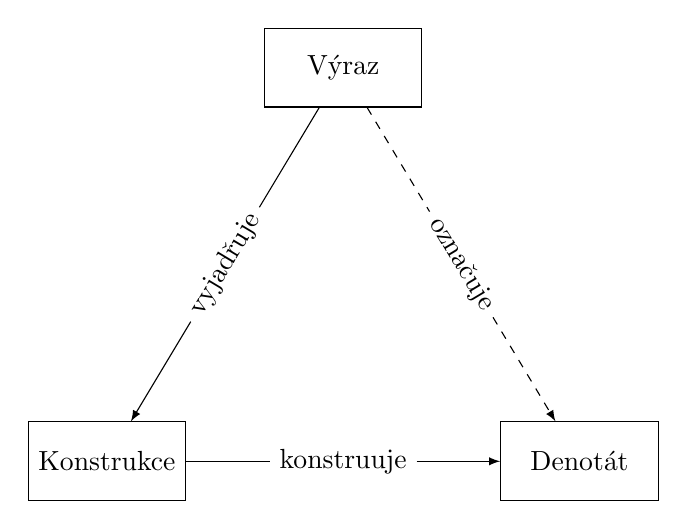
\begin{tikzpicture}
        \node[draw, fit={(0, 0) (2, 1)},              xshift=3cm, inner sep=0pt, label=center:Výraz] (A) {};
        \node[draw, fit={(0, 0) (2, 1)}, yshift=-5cm,             inner sep=0pt, label=center:Konstrukce] (B) {};
        \node[draw, fit={(0, 0) (2, 1)}, yshift=-5cm, xshift=6cm, inner sep=0pt, label=center:Denotát] (C) {};

        \path (A) -- node[sloped] (ab) {vyjadřuje}  (B);
        \path (A) -- node[sloped] (ac) {označuje}   (C);
        \path (B) -- node[sloped] (bc) {konstruuje} (C);

        \draw [-latex]          (A)--(ab)--(B);
        \draw [-latex] [dashed] (A)--(ac)--(C);
        \draw [-latex]          (B)--(bc)--(C);
    \end{tikzpicture}
    \caption{Schéma procedurální sémantiky TIL}\label{fig:til-semantics}
\end{figure}

Denotátem výrazu může být nejen objekt z báze, ale i konstrukce nebo funkce.

Jak již bylo zmíněno, Transparentní intenzionální logika vychází z typovaného lambda kalkulu, proto
také každý objekt musí mít svůj typ. Pro správné pochopení TILu, a tedy i této práce, je tak nutné 
znát typovou hierarchii TIL.

\section{Objektová báze}

Objektová báze je kolekce vzájemně disjunktních neprázdných množin, které dohromady vymezují
nulární funkce, se kterými budeme pracovat. Bázi volíme dle potřeb konkrétní aplikace a univerza
diskurzu. Například používáme-li TIL k logické analýze matematických vět, jako bázi lze zvolit
například množinu celých čísel, množinu reálných čísel, a množinu pravdivostních hodnot. Musíme
však vzít v potaz, že tato báze neobsahuje čísla komplexní.

Patří-li objekt $x$ do množiny $\alpha$ z báze, říkáme, že se jedná o objekt typu $\alpha$.
K explicitnímu uvedení typu objektu \textit{x} využíváme zápis $x/\alpha$. Množinám tvořícím bázi
lze přirozeně říkat typy.

Pro analýzu přirozeného jazyka se většinou volí objektová báze skládající se z typů {$o$, $\iota$,
$\tau$, $\omega$}. Tyto typy jsou podrobněji popsány v tabulce \peteref{tab:default-base}.

\begin{table}
    \caption{Výchozí báze pro analýzu přirozeného jazyka}\label{tab:default-base}
    \centering

    \begin{tabular} { | l l | }
        \hline
        Typ      & Popis typu \\
        \hline
        $o$      & Množina pravdivostních hodnot \\
        $\iota$  & Množina individuí (univerzum diskurzu) \\
        $\tau$   & Množina časových okamžiků/reálných čísel \\
        $\omega$ & Množina logicky možných světů \\
        \hline
    \end{tabular}
\end{table}

\section{Funkce}\label{fn-arity}

V některých logických systémech, například v predikátové logice, se jako základní molekulární typ
využívají relace. Funkce je poté speciální typ relace, která je zprava jednoznačná. V TIL je však
základním molekulárním typem funkce. Chceme-li v TIL vyjádřit $n$-ární relaci nad množinou
$\alpha_1 \times ... \times \alpha_n$, lze tak samozřejmě udělat definicí $n$-ární funkce
z $\alpha_1 \times ... \times \alpha_n$ do $o$, která každému prvku
z $\alpha_1 \times ... \times \alpha_n$ přiřadí pravdivostní hodnotu na základě toho, zda prvek
do relace patří, nebo ne.

% TODO: https://www.phil.muni.cz/~raclavsky/texty/partiality_til.pdf
Narozdíl od tradičního lambda kalkulu je Transparentní intenzionální logika kalkulem parciálních
funkcí. Z parciality funkcí poté vyplývá další vlastnost TIL -- arita funkcí není shora omezená.
V lambda kalkulech totálních funkcí lze využít Sch{\"o}nfinkelovu redukci k redukci funkcí
$n$-árních na unární za využití skládání funkcí. Tato redukce však není ekvivalentní, pracujeme-li
s funkcemi parciálními.

\subsection{Intenze a extenze}

V TIL dále rozlišujeme funkce na tzv. \textit{intenze} a \textit{extenze}. Intenze jsou funkce
z možných světů. Extenze jsou funkce, jejichž doménou množina možných světů není, a tudíž jejich
funkční hodnota nezávisí na stavu světa.

Intenze jsou obecně funkce typu $(\alpha\omega)$ pro libovolný typ $\alpha$. Nejčastěji se však
jedná o funkce typu $((\alpha\tau)\omega)$, tedy funkce zobrazující možné světy do chronologií
objektů typu $\alpha$.

\section{Konstrukce TIL}

Konstrukce v Transparentní intenzionální logice jsou abstraktní procedury. Tyto procedury jsou
strukturované -- nejedná se o množiny, mají pevně danou strukturu, a na uspořádání případných
podprocedur záleží. Tyto konstrukce lze podle definovaných pravidel provést. Provedením konstrukce
získáme výstup, případně nezískáme nic. Konstrukce, které nekonstruují žádný výstup, nazýváme
\textit{nevlastní} (anglicky \textit{improper}). V TIL pracujeme s šesti druhy konstrukcí.

Jak již bylo zmíněno, konstrukce můžou v TIL operovat nejen nad objekty, které nejsou konstrukcemi,
tedy nad objekty z báze a funkcemi, ale také nad jinými konstrukcemi. Konstrukce však může operovat
pouze nad konstrukcemi nižšího řádu, než je konstrukce samotná, viz \peteref{type-order}. Každou
podkonstrukci, kterou musíme provést při provedení konstrukce, nazýváme \textit{konstituentem}.
V TIL existuje šest různých druhů konstrukcí. Dvě atomické -- mají pouze jeden konstituent, a to
sebe samotné, a čtyři molekulární. Atomickými konstrukcemi jsou \textit{Trivializace} a
\textit{proměnné}. Mezi molekulární konstrukce poté řadíme \textit{Kompozice}, \textit{Uzávěry},
\textit{Provedení} a \textit{Dvojí Provedení}.

\textit{Proměnné} jsou konstrukce, které na základě valuace \textit{v} \textit{v}-konstruují
objekty. Skutečnost, že proměnná $x$ \textit{v}-konstruuje hodnotu typu $\alpha$ značíme
$x \rightarrow_v \alpha$.

\lstset{language=Lisp}
\textit{Trivializace} pro libovolný objekt \textit{X} konstruuje samotný objekt \textit{X}.
Konstrukce je v Transparentní intenzionální logice potřebná, neboť výchozím módem pro konstrukce
je provedení. Samotná konstrukce \textit{X} by tak byla automaticky provedena, a místo konstrukce
\textit{X} bychom dostali pouze její denotát. Pokud bychom chtěli zkonstruovat konstrukci
\textit{X}, musíme ji trivializovat. Tím se provede pouze konstrukce Trivializace. A protože
Trivializace nemá jiný konstituent, než sebe samotnou, konstrukce \textit{X} se tak neprovede.
V literatuře se Trivializace \textit{X} tradičně značí ${}^0X$. Alternativně se používá také zápis
$'X$. Tento zápis je poté využit i v jazyce TIL-Script. Trivializaci lze považovat za ekvivalent
funkce \lstinline{QUOTE} z jazyka Lisp. Trivializace taktéž bývá využívána ke konstruování hodnot,
které nelze provést (objekty z báze, funkce) a tudíž je nelze zmínit netrivializované.
\footnote{
    V jazyce Lisp čísla konstruují sebe samotné, tedy provedením čísla získáme zpět prováděné
    číslo. \lstinline{1} a \lstinline{'1} jsou tedy v Lispu ekvivalentní výrazy. V TIL však není
    možné, aby objekt konstruoval sám sebe, viz rozvětvená hierarchie typů \peteref{type-order}.
}

\textit{Kompozice} je procedura aplikace funkce na argumenty. Kompozice $[X Y_1...Y_m]$ značí
aplikaci funkce konstruované konstrukcí $X$ na argumenty zkonstruované konstrukcemi $Y_1,...,Y_m$.
Pokud konstrukce $X$ $v$-konstruuje funkci $f$, všechny podkonstrukce $Y_1,...,Y_m$ $v$-konstruují
hodnotu, a je-li funkce $f$ na daných argumentech definovaná, kompozice $v$-konstruuje funkční
hodnotu na těchto argumentech. V opačném případě je kompozice $v$-nevlastní.

\textit{Uzávěr} $\lambda x_1...x_m Y$ je konstrukce $v$-konstruující funkci. $x_1,...x_m$ musí
být navzájem různé proměnné, $Y$ musí být konstrukcí. Konstruce uzávěru je velmi podobná abstrakci
v lambda kalkulu. Narozdíl od lambda kalkulu však v TILu může uzávěr konstruovat funkce s aritou
vyšší než jedna. Uzávěr nemůže být nikdy nevlastní, může však konstruovat tzv.
\textit{degenerovanou funkci}, tedy funkci, která je nedefinovaná na celém definičním oboru.

\textit{Provedení} ${}^1X$ je konstrukce $v$-konstruující objekt konstruovaný konstrukcí $X$.
Pokud je konstrukce $X$ $v$-nevlastní, je provedení ${}^1X$ také $v$-nevlastní. Jelikož je však
provedení výchozím módem pro objekty, většinou se neuvádí. Provést lze pouze konstrukce. Objekty
z báze (tedy čísla, individua, apod...) či funkce nelze provést, jejich provedení nekonstruuje nic.
Proto je potřeba tyto objekty vždy trivializovat.

\textit{Dvojí provedení} ${}^2X$ je poslední z výčtu konstrukcí. Je-li $X$ konstrukcí
$v$-konstruující konstrukci $Y$, a $v$-konstruuje-li konstrukce $Y$ objekt $Z$, pak ${}^2X$
$v$-konstruuje $Z$. V opačném případě je dvojí provedení ${}^2X$ $v$-nevlastní.

Jiné konstrukce v Transparentní intenzionální logice neexistují.

\subsection{Princip kompozicionality} 

Princip kompozicionality je důležitým rysem Transparentní intenzionální logiky. Z principu
kompozicionality vyplývá, že je-li libovolný konstituent konstrukce $X$ $v$-nevlastní a pro danou
valuaci $v$ nekonstruuje žádnou hodnotu, pak je $v$-nevlastní i konstrukce $X$.

\section{Typy 1. řádu}\label{fst-order}

% TODO: Doplnit citaci
Definice je skoro slovo od slova převzata z knihy
\textit{TIL jako procedurální logika -- Průvodce zvídavého čtenáře Transparentní intensionální
logikou}. Tato sekce slouží jako krátké vysvětlení základů Transparentní intenzionální logiky
se čtenář může obrátit například na tuto knihu.

Nechť \textit{B} je báze. Pak:

\begin{enumerate}[i)]
    \item Každá množina z báze \textit{B} je atomický typ řádu 1 nad \textit{B}.
    \item Nechť $\alpha, \beta_1, ...,\beta_m (m > 0)$ jsou typy řádu 1 nad \textit{B}. Pak soubor
        všech \textit{m}-árních parciálních funkcí $(\alpha\beta_1...\beta_m)$, tedy zobrazení z 
        $\beta_1 \times ... \times \beta_m$ do $\alpha$, je molekulární typ řádu 1 nad \textit{B}.
    \item Nic jiného není typem řádu 1 nad bází \textit{B}.
\end{enumerate}

\section{Rozvětvěná hierarchie typů}\label{type-order}

%TODO: Doplnit citaci
Definice je opět skoro slovo od slova převzata z Průvodce.

Nechť \textit{B} je báze. Pak:

\subsection{$T_1$ (typy řádu 1)}
Viz sekce \peteref{fst-order}.

\subsection{$C_n$ (konstrukce řádu n)}

\begin{enumerate}[i)]
    \item Nechť $x$ je proměnná $v$-konstruující objekt typu řádu $n$. Pak $x$ je
        \textit{kontrukce řádu n nad B}.
    \item Nechť $X$ je prvek typu řádu $n$. Pak trivializace ${}^0X$, provedení ${}^1X$ a dvojí
        provedení ${}^2X$ jsou \textit{konstrukcemi řádu n nad B}.
    \item Nechť $X, Y_1, ... Y_m$ jsou konstrukce řádu $n$ nad \textit{B}. Pak kompozice 
        $[X Y_1...Y_m]$ je \textit{konstrukce řádu n nad B}.
    \item Nechť $x_1,...,x_m$ jsou vzájemně různé proměnné a $X$ je konstrukce řádu $n$
        nad \textit{B}. Pak uzávěr $[\lambda x_1 ... x_m X]$ je \textit{konstrukce řádu n nad B}.
    \item Nic jiného není konstrukcí řádu $n$ nad bází \textit{B} než dle i)-v).
\end{enumerate}

\subsection{$T_{n+1}$ (typy řádu n+1)}

Nechť $*_n$ je kolekce všech konstrukcí řádu $n$ nad $B$.

\begin{enumerate}[i)]
    \item $*_n$ a každý typ řádu $n$ jsou \textit{typy řádu n+1 nad B}.
    \item Jsou-li $\alpha, \beta_1,...,\beta_m$ typy řádu $n+1$ nad \textit{B}, pak
        $(\alpha \beta_1...\beta_m)$, tedy kolekce parciálních funkcí, je
        \textit{typy řádu n+1 nad B}.
    \item Nic jiného není typ řádu $n+1$ nad \textit{B} než dle i) a ii).
\end{enumerate}

% \section{Charakteristické rysy TIL}

% \subsection{Princip kompozicionality}

% Princip kompozicionality říká, že význam výrazu je jednoznačně určen významy jeho podsložek.
% Z principu kompozicionality také vyplývá, že nemá-li konstrukce žádný význam (tedy jedná se o
% nevlastní konstrukci), nemají význam ani konstrukce, pro něž je daná nevlastní konstrukce
% konstituentem.

% \subsection{Antikontextualismus}

% Antikontextualismus znamená, že význam výrazu je stejný nezávisle na stavu světa.

% \subsection{Antiaktualismus}

\section{Analytické a empirické výrazy}

Výrazy přirozeného jazyka lze dělit na dva typy výrazů, a to empirické a analytické.

Analytické výrazy jsou výrazy takové, které označují extenze nebo konstantní intenze. Jedná se
například o matematické věty nebo věty vyjadřující relaci rekvizity mezi vlastnostmi (např. věta
``Všechny velryby jsou savci'' je analytická a nutně pravdivá nezávisle na stavu světa, neboť
existuje-li individuum, které je velrybou, pak bude vždy také savcem.)

Empirické výrazy naopak označují intenze, jejichž hodnota na stavu světa závisí. Abychom určili
hodnotu dané intenze, musíme empiricky zkoumat stav světa v daném časovém okamžiku. Empirické
zkoumání světa ovšem již není záležitost logiky.
\endinput

\chapter{TIL-Script}\label{tilscript-chapter}

Nyní konečně přišel čas představit TIL-Script. TIL-Script je interpretovaný funkcionální
programovací jazyk, do znatelné míry inspirovaný jazyky jako Haskell nebo Lisp. Syntax jazyka
TIL-Script by měla co nejvíce připomínat syntaktické prvky Transparentní intenzionální logiky, aby
pouhá znalost TILu stačila k okamžitému pochopení jazyka TIL-Script. Sémantika TIL-Script konstrukcí
poté musí odpovídat sémantice TIL.

Tato kapitola je rozdělena do tří sekcí. V první sekci jsou popsány důležité základní rysy jazyka
TIL-Script. Druhá sekce popisuje již existující jazykové prvky, případně také dokumentuje změny
oproti předchozím iteracím jazyka. Poslední sekce navrhuje rozšíření jazyka TIL-Script.

\section{Charakteristické rysy jazyka TIL-Script}

Tato sekce popisuje charakteristické rysy jazyka TIL-Script v takové podobě, jakou nabývá v této
práci. Pokud se v některém bodě TIL-Script neshoduje s TILem či předchozími verzemi jazyka
TIL-Script, je rozdíl náležitě popsán a vysvětlen.

\subsection{Lambda kalkul parciálních funkcí}

\subsubsection{Shora neomezená arita funkcí}

% TODO: Ozdrojovat currying asi? Idk, lambda kalkul

Na rozdíl od lambda kalkulu ve své tradiční podobě, nebo například jazyka Haskell, v Transparentní
intezionální logice není arita funkce shora omezená, viz \peteref{fn-arity}. TIL-Script musí tento
fakt reflektovat. Proto tento jazyk umožňuje definici i aplikaci funkcí libovolné (samozřejmě
kladné) arity. Nevyužíváme zde tedy rozvíjení funkcí (anglicky \textit{currying}). Zatímco např.
v Haskellu jsou funkce arity dvě nebo vyšší automaticky rozvinuty na sérií několika unárních
funkcí, jejichž oborem hodnot jsou unární nebo nulární funkce, v jazyce TIL-Script není arita nijak
omezená.

\subsubsection{Parciální funkce a respektování principu kompozicionality}

Jelikož v TIL můžou být funkce parciální, musí i TIL-Script počítat s parcialitou funkcí. Dále musí
TIL-Script respektovat princip kompozicionality, základní rys Transparentní intenzionální logiky.
Jedním z důsledků principu kompozicionality je, že konstrukce, jejíž přinejmenším jeden konstituent
je $v$-nevlastní, bude také nutně $v$-nevlastní. Reprezentaci stavu, kdy je parciální funkce
aplikována na argumenty, na kterých není definována, se věnuje podsekce \peteref{nil-value}
této kapitoly. 

%TODO: Ocitovat
Jedinou výjimkou je funkce \lstinline{IsNil}, jež vrací pravdivostní hodnotu \lstinline{True},
pokud je její jediný argument \lstinline{Nil}, v opačném případě je jejím výsledkem
\lstinline{False}. Tato speciální sémantika funkce \lstinline{IsNil}, ačkoliv porušuje princip
kompozicionality a vyžaduje aplikaci unární funkce na \textit{nic}, je zvolena jako doplněk
k funkci $Improper/(o*_n)$ definované v Průvodci čtenáře, a jako kompromis mezi dodržením
principů TIL a umožněním zpracování chybových stavů.

%TODO: Pokračovat v kontrole

\subsection{Okamžité vyhodnocování}

Ačkoliv je TIL-Script funkcionální jazyk, vyhodnocování výrazů probíhá okamžitě
(tzv. \textit{Eager evaluation}). Okamžité vyhodnocování je potřeba k zajištění respektování
principu kompozicionality. Pokud by vyhodnocování bylo líné, programátor implementující TIL-Script
funkci v jazyce Java by si mohl vyžádat vyhodnocení argumentu během aplikace funkce, zjistit,
že funkce neobdržela jeden z argumentů, ale přesto by mohl tento fakt ignorovat a vrátit ze své
funkce validní hodnotu. Tím by však došlo k aplikaci funkce na chybějící argument a také k porušení
principu kompozicionality (konstrukce by mohla mít význam, ačkoliv je jedna z jejích konstrukcí
$v$-nevlastní).

\subsection{Neměnnost argumentů funkcí a objektů (\textit{Immutability})}

Jelikož je TIL-Script funkcionální jazyk, jsou objekty a argumenty funkcí neměnné
(\textit{immutable}). Zatímco v imperativních jazycích, jako je třeba jazyk C++, není problém
v těle funkce modifikovat argument, který funkce obdržela, v jazyce TIL-Script nic takového provést
nemůžeme. Dále například nemůžeme modifikovat existující seznam. Pokud chceme transformovat již
existující seznam, musíme vytvořit nový seznam a požadované hodnoty uložit v novém seznamu. Podobně
nemůžeme změnit hodnoty n-tice, můžeme však vytvořit novou n-tici.

Hodnotu volné proměnné změnit lze, abychom mohli zkoumat konstrukce při různých valuacích $v$.
Typ proměnné však změnit nelze.

Obdobně nelze redefinovat funkce nebo změnit typ symbolické hodnoty
(viz \peteref{symbolic-values}).

\subsection{Definice a deklarace symbolů}

TIL-Script nově rozlišuje mezi deklaracemi a definicemi proměnných a funkcí. Deklarace pouze
uvědomí překladač o existenci proměnné nebo funkce, nijak ale nedefinuje valuaci proměnné nebo
sémantiku funkce. Deklarace umožňuje funkci či proměnnou zmínit (např. v trivializaci, v uzávěru),
neumožňuje nám však proměnnou provést nebo funkci aplikovat -- jak také, když neznáme hodnotu
proměnné, případně sémantiku dané funkce. Provedení deklarované, avšak nedefinované proměnné
je chybou, při které interpret ohlásí chybu a běh programu je ukončen. Deklarovat jeden symbol
lze vícekrát, deklarace však nesmí být konfliktní a lišit se typy.

\begin{lstlisting}[caption={Hlášení chyby při chybějící definici}]
$ java -jar interpreter/build/libs/tilscript.jar examples/undef-var.tils
** Error **
(4, 1): myVar.
    ~~~ ^ ~~~
        Variable 'myVar' is declared but undefined
$ java -jar interpreter/build/libs/tilscript.jar examples/undef-fn.tils
** Error **
(2, 1): MyFn/(Int Int Int).
    ~~~ ^ ~~~
        Function MyFn is declared but undefined, application is impossible
\end{lstlisting}

Definice přiřadí proměnné valuaci, funkci sémantiku. Proměnné s řádnou definicí lze provést
a můžou tak být konstituentem prováděné konstrukce. Funkce s řádnou definicí lze aplikovat. Funkce
i proměnné lze definovat pouze jednou. Opakovaná definice je chybou a vyústí v předčasné ukončení
programu.

Symbolické hodnoty, viz \peteref{symbolic-values}, lze pouze deklarovat.

Deklarace jsou automaticky odvozeny z definic. Proto, pokud je známa definice, není třeba dodávat
také deklaraci. K interpretaci deklarací automaticky dochází před interpretací definic, aby byla
umožněna např. definice vzájemně rekurzivních funkcí. Definice jsou interpretovány v takovém
pořadí, v jakém jsou uvedené ve zdrojovém kódu.

Deklarace bez řádných definic na první pohled můžou působit zbytečně. K čemu může sloužit funkce,
kterou nelze aplikovat? Nesmíme však zapomenout, že konstrukce TIL samy vyjadřují význam, a nemusí
nutně sloužit pouze k provedení. Provedením konstrukce sice dostaneme její denotát, ten nás ale ne
vždy zajímá. Představme si tedy případ, kdy provádíme analýzu výrazu přirozeného jazyka. Výraz
analyzujeme pomocí Transparentní intenzionální logiky a získáme konstrukci. S danou konstrukcí
chceme dále pracovat a chceme ji strojově zpracovat. Její denotát nás ovšem nezajímá, zajímá nás
pouze význam konstrukce -- procedura. Současně daná konstrukce obsahuje funkci, jejíž definici vůbec
neznáme, nebo ji známe, ale nejsme schopni ji strojově vyjádřit, nebo nás pouze nezajímá. Jelikož
víme, že konstrukci nebudeme provádět, a tedy nebudeme ani aplikovat funkci v ní zmíněnou,
nepotřebujeme znát její přesnou definici. Stačí nám znát pouze její název a typ.

Pro představu uveďme několik příkladů, kdy stačí dodat deklaraci (název a typ), protože
nepotřebujeme definici (název, typ i sémantiku).

Představme si situaci, kdy analyzujeme větu ``V minulosti se pro výpočet převrácené hodnoty druhé
odmocniny využívala funkce \textit{Fast Inverse Square Root}''. Jistě pro analýzu věty budeme
nutně potřebovat deklarovat funkci \lstinline{FastInvSqrt/(Real Real)}. Implementaci funkce
\textit{Fast Inverse Square Root} v jazyce C lze jednoduše nalézt na internetu. Tato funkce se však
již roky nevyužívá, neboť moderní procesory implementují výpočet druhé odmocniny i její převrácené
hodnoty hardwarově. Současně na první pohled vidíme, že funkci \lstinline{FastInvSqrt} nebudeme
potřebovat aplikovat. Není tedy třeba na internetu dohledávat existující specifikaci funkce
\textit{Fast Inverse Square Root} a definovat danou funkci v jazyce TIL-Script. Současně pro výpočet
převrácené hodnoty druhé odmocniny čísla existují efektivnější metody, proto danou funkci
nepotřebujeme aplikovat ani v případě, kdy potřebujeme provést matematické operace (za předpokladu,
že např. nezkoumáme chybu této funkce). Rozlišení definic a deklarací zde slouží převážně k ušetření
práce.

Jako jiný příklad lze uvést tzv. \textit{Halting problem}, tedy algoritmicky nerozhodnutelný
problém, zda program někdy zastaví. Jistě si lze představit matematickou funkci, která rozhodne,
zda program zastaví. Můžeme například seřadit všechny syntakticky korektní programy dle abecedy,
následně je očíslovat, a vytvořit nekonečnou tabulku, která každému programu přiřadí hodnotu 1,
pokud program zastaví, v opačném případě pak hodnotu 0. Jelikož však počítače mají pouze omezené
zdroje, nekonečnou tabulku sestavit nelze. A jelikož, jak dokázal již Alan Turing, je tento problém
algoritmicky nerozhodnutelný, nemůžeme ani sestavit algoritmus, který obdrží na vstupu zdrojový kód,
a na základě analýzy zdrojového kódu rozhodne, zda program zastaví. Přesto však funkci
\lstinline{Zastaví/(Bool Text)}, případně \lstinline{Halts/(Bool Text)} můžeme potřebovat například
k analýze věty ``Programátor zkoumá, zda jeho program někdy zastaví.'' V tomto případě deklaraci bez
definice využijeme proto, že korektní definice funkce \lstinline{Halts/(Bool Text)} neexistuje.

Názvosloví \textit{deklarace}, \textit{definice} je převzato z programovacího jazyka C, kde
deklarace pouze uvědomí překladač o existenci symbolu, definice poté přiřadí symbolu konkrétní
hodnotu. Počet deklarací je shora neomezený, naopak definice může existovat nanejvýš jedna.
Deklarace nedefinovaného symbolu není chybou, ovšem snaha nedefinovaný symbol využít (např. volání
funkce, přístup k proměnné) vyústí v chybu při procesu linkování.

\section{TIL-Script jako výpočetní varianta TILu}

Tato sekce popisuje základní výrazy a konstrukce jazyka TIL-Script, které existovaly již
v předchozích verzích jazyka. Pokud práce tyto výrazy nějakým způsobem upravuje, je úprava náležitě
popsána a zdůvodněna.

\subsection{Věty jazyka TIL-Script}

V jazyce TIL-Script za věty (\textit{sentence}) považujeme výrazy na nejvyšší úrovni v programu.
Větou je tedy například konstrukce taková, že není podkonstrukcí jiné konstrukce než sebe samotné,
ale také definice funkce, proměnné, typu, apod. Každá věta musí být ukončena terminátorem. Roli
terminátoru zastává znak \lstinline{.} (tedy ASCII tečka).

\subsection{Atomické datové typy}

Atomické datové typy v jazyce TIL-Script vycházejí z výchozí báze využívané v Transparentní
intenzionální logice k analýze přirozeného jazyka, tedy z množin ${o, \iota, \tau, \omega}$. TIL-Script ovšem
rozlišuje mezi časy a reálnými čísly, a pro tyto hodnoty definuje dva nekompatibilní typy, mezi
kterými neexistuje implicitní konverze. Dále TIL-Script využívá typ $\nu$ představující celá
čísla. Nakonec TIL-Script pro názvy typů nevyužívá řecká písmena, která nelze prakticky a jednoduše
zapisovat na většině rozložení klávesnic, ale anglická slova nebo zkratky. Názvy typů vždy začínají
velkým písmenem.

Typ $o$ představující pravdivostní hodnoty TIL-Script pojmenovává \lstinline{Bool}. Hodnotami typu
\lstinline{Bool} jsou poté hodnoty \lstinline{True} a \lstinline{False}.

Typ $\iota$, v jazyce TIL-Script \lstinline{Indiv}, reprezentuje množinu individuí. Individua
v Transparentní intenzionální logice považujeme za \textit{holá} -- žádnou netriviální vlastnost
nemají nutně. Všechny netriviální vlastnosti individuí jsou určeny stavem světa. Individuum samotné
nemá žádnou inherentní valuaci. Slouží pouze jako unikátní indentifikátor. Obdobně hodnoty
\lstinline{Indiv} v jazyce TIL-Script nemají žádnou konkrétní reprezentaci. Typ \lstinline{Indiv}
je využíván v konjunkci se symbolickými hodnotami, viz \peteref{symbolic-values}. Tímto TIL-Script
umožňuje uživateli referovat na konkrétní individuum pouze pomocí symbolického identifikátoru,
aniž by individuím musely být přiřazeny arbitrárně zvolené konkrétní hodnoty.

Reálná čísla TIL-Script reprezentuje typem \lstinline{Real}. V implementaci překladače vytvořeném
v rámci této práce jsou reálná čísla interně reprezentována typem \lstinline{double}. TIL-Script
samotný žádné omezení na reprezentaci reálných čísel nestanovuje, prakticky však reálná čísla
v současné implementaci reprezentujeme pomocí 64bitové reprezentace dle IEEE 754.

Celá čísla TIL-Script reprezentuje typem \lstinline{Int}. Obdobně jako u typu \lstinline{Real}
neexistuje omezení pro reprezentaci celých čísel. Interně je využíván datový typ \lstinline{long},
jedná se tedy o 64bitové znaménkové číslo reprezentované dvojkovým doplňkem.

Množinu možných časů modelujeme typem \lstinline{Time}. Pro interní reprezentaci časových okamžiků
byl v této práci zvolen datový typ \lstinline{long}. Uživatel se sám může rozhodnout, jak bude tyto
hodnoty interpretovat. Ve standardní knihovně lze však nalézt např. funkci \lstinline{Now}, jejíž
aplikací získáme počet milisekund uplynulých od 1. ledna 1970.

Typ konstrukcí, v TIL denotován $*$, byl v jazyce TIL-Script přejmenován
na \lstinline{Construction}. V dřívějších verzích jazyka se pro typ konstrukcí také využíval znak
$*$. Změna na \lstinline{Construction} byla provedena z důvodu zachování konzistence s ostatními
typy, které v jazyce TIL-Script taktéž pojmenováváme anglickými slovy, a také z důvodu omezení
ambiguity, aby se typ konstrukce nepletl s funkcí násobení. Zatímco typograficky korektní
reprezentací násobení je využití znaku $\times$, na počítači násobení značíme $*$. Ačkoliv lze mezi
funkcí násobení a typem konstrukcí odlišit na základě kontextu, v jakém se znak objevuje, odlišení
již v názvu umožňuje uživateli jednoduše rozeznat typ konstrukce od násobení čísel okamžitě a
bez bližšího zkoumání kontextu.

Dále byl TIL-Script rozšířen o atomický typ sloužící k reprezentaci textu. Tento typ je podrobněji
popsán v sekci o rozšířeních jazyka, viz \peteref{text-type}.

\subsection{Generický typ \textit{Any}}

V Transparentní intenzionální logice není neobvyklé definovat typově polymorfní funkce. Zvykem je
označovat předem neznámé typy řeckým písmenem $\alpha$. Obdobně TIL-Script umožňuje definici
typově polymorfních funkcí. Generické typy v jazyce TIL-Script značíme slovem \lstinline{Any},
okamžitě následovaným indexem polymorfního typu. Index je libovolné číslo z rozsahu
$\bigl \langle 0; 2^{32}-1 \bigr \rangle$. Nenulové indexy nesmí začínat číslem 0.

Generické typy lze použít pouze v typech funkcí. Má-li více argumentů funkce stejný generický
typ, tedy typ \lstinline{Any} se stejným indexem, překladač při procesu typové kontroly zajistí,
že argumenty, na něž je funkce za běhu aplikována, jsou stejného typu.

\subsection{Výrazy \textit{TypeDef}}

Výrazy \lstinline{TypeDef} umožňují přiřadit již existujícímu typu alternativní jméno.
\lstinline{TypeDef} nevytváří nový typ, jedná se pouze o alternativní název. V průběhu typové
kontroly jsou tato jména rekurzivně přepisována, dokud překladač nezjistí původní typ. Teprve poté
porovnává původní typy, nezávisle na jejich alternativních názvech. Typové aliasy můžeme využívat
například pro zkrácení zápisu komplikovaných molekulárních typů. Obdobné zkratky v TIL využíváme
běžně.

Korektní syntaktický zápis \lstinline{TypeDef} výrazu začíná právě klíčovým slovem
\lstinline{TypeDef}, následovaným novým názvem, operátorem přiřazení \lstinline{:=}, a nakonec
původním typem. Název musí začínat velkým písmenem.

\begin{lstlisting}[caption={Výraz TypeDef}]
TypeDef Float := Real.
TypeDef Property := (((Bool Indiv) Time) World).
\end{lstlisting}

\subsection{Funkce}

V matematice známe funkce jako jednoznačné zobrazení z množiny možných argumentů (definiční obor)
do množiny možných obrazů (obor hodnot). V programovacích jazycích konstrukce nazývané funkcemi
často nemusí být nejen jednoznačné (výstup nemusí odpovídat pouze argumentům), ale dokonce nemusí
být ani zobrazením (nevrací žádnou hodnotu, v takovém případě většinou modifikují stav světa,
jako příklad lze uvést funkce s návratovou hodnotou \lstinline{void} v jazyce C).

V jazyce TIL-Script, obdobně jako v TIL, jsou funkce vždy zobrazením do určitého oboru hodnot. Díky
parcialitě může být funkce degenerovaná, a v takovém případě nebude vracet hodnotu pro žádnou
kombinaci argumentů. V takovém případě se však jedná o určitou formu chybového stavu, spíše než
záměr, jak by tomu bylo v případě např. jazyka C.

Implementací TIL-Script funkce v jazyce Java lze vytvořit TIL-Script funkci, která bude modifikovat
stav světa např. zápisem do databáze. Ačkoliv tomuto nelze zabránit, je na zvážení uživatele, zda
je TIL-Script, tedy nástroj pro logickou analýzu přirozeného jazyka, také vhodný nástroj pro plnění
databáze.

Arita funkce musí být vždy alespoň jedna.

Pro zápis typu funkce využíváme podobnou notaci jako v Transparentní intenzionální logice.
Typy funkcí denotujeme kulatými závorkami. Uvnitř závorek uvedeme nejprve obor hodnot funkce,
poté uvádíme postupně typy argumentů. Jediný rozdíl oproti TIL spočívá v nutnosti zapsat mezeru
mezi názvy jednotlivých typů. Tedy ekvivalentem k typu $(o\nu\tau)$ by v jazyce TIL-Script byl typ
\lstinline{(Bool Int Real)}, případně \lstinline{(Bool Int Time)}.

Funkce lze deklarovat uvedením názvu funkce následovaným lomítkem a jejím typem. Deklarujeme-li
více funkcí stejného typu, můžeme uvést více názvů oddělených čárkami. Pro definici funkce byla
přidána nová syntax popsaná v sekci \peteref{fn-definition}.

\begin{lstlisting}[caption={Deklarace funkcí}]
Add, Sub, Mult, Div/(Int Int Int).
\end{lstlisting}

\subsection{Literály}

Názvosloví \textit{literál} je přejato z jiných programovacích jazyků. V jazyce TIL-Script literály
myslíme ne-funkce, tedy členy množin tvořících bázi. Pomocí literálů lze uvádět celá i reálná
čísla, pravdivostní hodnoty, a také text (viz oddíl \peteref{text-type} věnující se typu
\lstinline{Text}). Individua zmiňujeme pouze za využití symbolických hodnot, viz Symbolické hodnoty
\peteref{symbolic-values}. Literály nikdy nesmíme zapomenout trivializovat.

\subsection{Trivializace}

Trivializace v jazyce TIL-Script slouží ke stejnému účelu jako v Transparentní intezionální logice.
Na rozdíl od TIL ovšem Trivializaci denotujeme apostrofem, namísto nuly zapsané jako levý horní
index.

\begin{lstlisting}[caption={Příklad Trivializace.}]
'1          -- Trivializace konstanty typu Int
'3.14159    -- Trivializace konstanty typu Real
'['+ '1 '2] -- Trivializace kompozice
\end{lstlisting}

\subsection{Proměnné}

Proměnné v jazyce TIL-Script opět slouží stejnému účelu jako proměnné v TIL, tedy $v$-konstruují
hodnotu v závislosti na valuaci $v$.

Volné proměnné lze deklarovat bez přiřazení valuace, ale lze je také definovat a přiřadit jim
konkrétní hodnotu. Proměnné deklarujeme, pokud nás nezajímá konkrétní valuace. Přiřazení hodnoty
využijeme například v případě, kdy si chceme uložit výsledek drahé operace (např. čtení
z databáze), nebo si třeba jen chceme zkrátit zápis dlouhé konstrukce, a chceme pracovat
s konkrétní valuací $v$. Vždy je třeba uvést typ hodnoty, kterou proměnná konstruuje.

% Je-li konstrukce, jejíž hodnotu přiřazujeme proměnné, $v$-nevlastní,
% a tedy nekonstruuje žádnou hodnotu, program skončí chybou.

Syntax pro deklaraci proměnné již existovala. Syntax pro definici proměnné (přiřazení hodnoty)
je nově zavedená. Deklarovat můžeme více proměnných najednou, za předpokladu, že se jedná o
proměnné stejného typu, stačí názvy jednotlivých proměnných oddělit čárkou. Přiřazujeme-li však
proměnné valuaci, můžeme uvést vždy pouze jednu proměnnou.

Pro změnu hodnoty volné proměnné použijeme stejnou syntax jako při úvodním přiřazení hodnoty.
Přiřazení hodnoty proměnné však není konstrukce, ale metavýraz, proto lze hodnotu proměnné vždy
změnit pouze na nejvyšší úrovni v programu. Typ proměnné změnit nelze.

Deklarace proměnných jsou vždy provedeny hned po spuštění programu, nezávisle na tom, kde v programu
jsou uvedeny. Přiřazení hodnot proměnným není prováděno přednostně, aby byla umožněna korektní
redefinice proměnné. Hodnota proměnné je tehdy změněna pouze a přesně na místě, kde je tak uvedeno
v programu. Deklarace jsou však z definic vždy dedukovány automaticky -- proměnná je přednostně
deklarována při spuštění programu, i když její deklarace není uvedena explicitně.

Název proměnné musí začínat malým písmenem. 

\begin{lstlisting}[caption={Příklad využití proměnných}]
x -> Int.               -- Deklarace proměnné v-konstruující hodnotu typu Int
y, z -> Int.            -- Deklarace více proměnných najednou
pi -> Real := '3.1415.  -- Definice proměnné pi aproximující hodnotu pi
['* pi '2].             -- Využití proměnné pi jako konstituent konstrukce
long_varName123 -> Int.
\end{lstlisting}

\subsection{Provedení}

Provedení se sémantikou opět nijak neliší od svého ekvivalentu v Transparentní intenzionální
logice. Syntax ovšem musela být kvůli praktičnosti upravena, a proto bylo upuštěno od pravých
horních indexů. Provedení denotujeme \lstinline{^1}. Pro Dvojí Provedení poté využíváme
\lstinline{^2}. Dřívejší verze jazyka TIL-Script definovaly i trojí až deváté Provedení. Protože
však trojí a vícenásobné provedení není v praxi skoro vůbec potřeba (dle Průvodce TIL taková potřeba
nenastala), a protože limit devátého Provedení byl poněkud arbitrární (proč ne například
desetinásobné Provedení), je tato práce konzervativní a drží se definice Provedení z Průvodce.

Jelikož jsou všechny konstrukce standardně v módu Provedení, není třeba explicitní Provedení
využívat příliš často. Většinou tedy budeme používat Dvojí Provedení.

\begin{lstlisting}[caption={Příklad využití Provedení}]
^1 x.
^2['GetComposition argument1 argument2].
\end{lstlisting}

\subsection{Kompozice}

Kompozice umožňuje aplikovat funkce na argumenty. Kompozice využívají stejnou syntax jako v TIL.
Protože arita funkce musí být alespoň jedna, musí i Kompozice obsahovat alespoň dvě podkonstrukce
-- funkci samotnou a alespoň jeden její argument. Počet argumentů, na něž funkci aplikujeme, musí
odpovídat počtu argumentů funkce. Dále nesmí být žádný argument $v$-nevlastní (s výjimkou funkcí
\lstinline{If} a \lstinline{IsNil}). V opačném případě k aplikaci funkce vůbec nedojde, neboť
nemáme argumenty, na které bychom funkci aplikovali, a Kompozice je tak $v$-nevlastní.

\begin{lstlisting}[caption={Příklad využití Kompozice}]
['* '2 '6].
\end{lstlisting}

\subsection{Uzávěry}

Sémantika Uzávěrů je opět stejná jako v Transparentní intenzionální logice, syntax ovšem byla
upravena. Zatímco v TIL často vypouštíme hranaté závorky, v jazyce TIL-Script musíme závorky zapsat
vždy. Řecké písmeno lambda nahradil v jazyce TIL-Script znak zpětného lomítka.

Zpětné lomítko následuje seznam argumentů funkce konstruované Uzávěrem. V dřívějších verzích jazyka
TIL-Script bylo možné typ argumentu v některých případech vynechat -- existovala-li volná proměnná
se stejným názvem jako $\lambda$-vázaná proměnná v Uzávěru, a nebyl-li typ $\lambda$-vázané
proměnné uveden explicitně, byl typ $\lambda$-vázané proměnné automaticky dedukován podle typu
stejnojmenné volné proměnné. Tato práce však od této automatické dedukce upouští. Jelikož byly
do jazyka TIL-Script přidány výrazy \lstinline{Import} umožňující importovat volné proměnné z jiného
souboru, uživatel jazyka by se mohl dostat do situace, kdy musí procházet několik
importovaných souborů, jen aby zjistil typ $\lambda$-vázané proměnné. V případě, kdy máme více
$\lambda$-vázaných proměnných, použijeme čárku pro jejich oddělení.

Za seznamem argumentů může nově následovat explicitní specifikace oboru hodnot konstruované funkce.
Specifikaci oboru hodnot denotujeme symbolem \lstinline{->}, který následuje název existujícího
typu. Explicitní specifikace je nepovinná, může však sloužit k zdůraznění úmyslu uživatele, aby
čtenář zdrojového kódu na první pohled znal typ funkce. Dále explicitní specifikace typu může
pomoct při typové kontrole.

Nakonec je třeba uvést konstrukci, nad kterou abstrakci provádíme.

\begin{lstlisting}[caption={Příklad využití Uzávěrů}]
[\x: Int -> Int ['+ x '2]].
[\x: Int, y: Int -> Int ['+ x y]].
[\x: Int, y: Int ['+ x y]].

[[\x: Int, y: Int -> Int ['+ x y]] '2 '3].
\end{lstlisting}

\subsection{Zkrácený zápis typu intenzí a extenzionalizace}

V TIL často využíváme zkráceného zápisu jak pro typy intenzí, tak pro jejich extenzionalizaci.
Pro hodnoty typu $\alpha$ závislé na světamihu zkracujeme zápis $((\alpha\tau)\omega)$
na $(\alpha_{\tau\omega})$. Obdobně pro extenzionalizaci intenze $a$ využíváme zkráceného zápisu
$a_{wt}$ ekvivalentnímu konstrukci $[[a w] t]$, kde $a$ je konstrukce konstruující funkci
(většinou se jedná o Trivializaci), a $w \rightarrow_v \omega$, $t \rightarrow_v \tau$. Jedná
se však pouze o notační zkratku -- o dohodu, ne součást TIL.

Ekvivalentní zkratky můžeme využívat také v jazyce TIL-Script. Chceme-li specifikovat typ intenze,
můžeme využít notační zkratku \lstinline{@tw}. Zkratku \lstinline{@wt} využijeme k extenzionalizaci
intenze. Zkratka \lstinline{@wt} vždy extenzionalizuje za využití proměnných \lstinline{w} a
\lstinline{t}. Proměnná \lstinline{w -> World} je součástí standardní knihovny, proměnnou
\lstinline{t -> Time} musí uživatel definovat sám. Zkrácenou notaci nelze využít s proměnnými
jiného názvu.

\begin{lstlisting}[caption={Příklad využití zkrácené notace}]
(Bool Indiv)@tw -- intenze typu (((Bool Indiv) Time) World)
['Rektor@wt 'VSB] -- extenzionalizace funkce Rektor/(((Indiv Indiv) Time) World)
                  -- a následná aplikace na argument VSB.
\end{lstlisting}

\subsection{Seznamy}

Seznamy se v Transparentní intenzionální logice příliš neobjevují. Při strojové analýze a
zpracování je však vhodné mít k dispozici způsob vyjádření kolekce dat, proto TIL-Script seznamy
obsahuje. Seznam představuje homogenní seřazenou kolekci potenciálně neomezené délky. Seznamy můžou
obsahovat duplicity.

% TODO: Lisp ref
V této práci jsou všechny seznamy neměnné. Seznamy jsou definovány induktivně. Seznam je buď
prázdný seznam, nebo \textit{cons cell} skládající se z hlavičky (známé jako \textit{head} nebo
\textit{CAR} z jiných jazyků) -- prvního prvku v seznamu, a z podseznamu reprezentujícího
zbytek seznamu (\textit{tail}, \textit{CDR}). Z definice tedy vyplývá, že vytvoření nového seznamu
vložením prvku na začátek lze provést v konstantním čase. Vytvoření nového seznamu přidáním prvku
na konec jiného seznamu naopak bude lineární vzhledem k velikosti původního kolekce. Tato
implementace seznamu je volena zejména proto, že umožňuje snadnou iteraci pomocí rekurzivních funkcí.
Stejnou implementaci seznamů využívají například jazyky Lisp, Haskell, a další.

Typ seznamu denotujeme slovem \lstinline{List} následovaným kulatými závorkami, v nichž je uveden
typ prvku ukládaného v seznamu.

% TODO: Ref to stdlib documentation
Standardní knihovna obsahuje řadu funkcí pro práci se seznamy. Tyto funkce jsou v této kapitole
pouze nastíněny při ilustraci využití seznamů, podrobněji jsou však zdokumentovány v kapitole
popisující standardní knihovnu.

Dále interpret implementuje syntaktický cukr pro jednodušší vytváření seznamů. Pro vytvoření
seznamu stačí v kompozici aplikovat funkci \lstinline{ListOf} na nenulový, avšak shora neomezený
počet argumentů. Během parsování bude tato kompozice korektně přepsána na sérii kompozic
využívajících funkci \lstinline{Cons} k vytvoření \textit{cons cells}. K žádné aplikaci funkce
na libovolný počet argumentů tedy nedochází. Při vytváření seznamu pomocí \lstinline{ListOf} musíme
dodat alespoň jeden prvek seznamu, aby bylo možné správně dedukovat typ prvků ukládaných v seznamu.
\lstinline{ListOf} je pouze syntaktický cukr překládaný při procesu parsování. Pokud bychom chtěli
generovat konstrukce konstruující seznamy dynamicky za běhu programu, museli bychom zřetězit
aplikace \lstinline{Cons}.

\begin{lstlisting}[caption={Příklad využití seznamů}]
['ListOf '1 '2 '3].                    -- vytvoření seznamu
['Cons '1 ['Cons '2 ['ListOfOne '3]]]. -- ekvivalent předchozího řádku
                                       -- a ukázka přepisu ListOf
['Head ['ListOf '1 '2 '3]]             -- 1
['Tail ['ListOf '1 '2 '3]]             -- ['ListOf '2 '3]
\end{lstlisting}

\subsection{N-tice}

N-tice doznaly oproti předchozím verzím jazyka TIL-Script změny. Dříve byly n-tice homogenní kolekce
nespecifikované, avšak konečné délky. Roli homogenní kolekce však již zastává List, a v jazyce
TIL-Script neexistoval způsob, jak seskupit více hodnot jiného typu dohromady.

V matematice využíváme n-tice například k reprezentaci prvků kartézského součinu. N-tice lze
definovat více způsoby, vždy jsou však uspořádané, konečné, a můžou být heterogenní (například
pokud provádíme kartézský součin nad neidentickými množinami). Obdobnou roli plní n-tice i v jazyce
TIL-Script. Délka n-tice je pevně daná, stejně jako typy hodnot v n-tici. Celý typ n-tice je
tedy dán uspořádaným výčtem všech typů všech hodnot obsažených v této n-tici. Syntaktický zápis
typu n-tice je podobný typu seznamu. Typ n-tice denotujeme slovem \lstinline{Tuple}, následovaným
kulatými závorkami. V závorkách ovšem uvádíme výčet typů. Jednotlivé typy oddělujeme čárkami. Délka
n-tice je určena počtem uvedených typů.

Práce s n-ticemi je do jisté míry podobná práci se seznamy. N-tici vytvoříme aplikací variadické
funkce \lstinline{MkTuple}. Stejně jako u funkce \lstinline{ListOf} se však jedná pouze o
syntaktický cukr. Funkce \lstinline{MkTuple} skutečně existuje, je to ale funkce binární, nikoliv
variadická, a vytváří dvojice z dodaných argumentů. Pokud ovšem funkci \lstinline{MkTuple} dodáme
více než dva argumenty, parser aplikaci \lstinline{MkTuple} rozepíše na jednu aplikaci
\lstinline{MkTuple} a následné řetězení funkce \lstinline{PrependToTuple}. Funkce pro práci
s n-ticemi jsou podrobněji popsány v uživatelské dokumentaci.
 
\begin{lstlisting}[caption={Příklad využití n-tic}]
['MkTuple '1 '2.0 'True].                    -- vytvoření n-tice
['PrependToTuple '1 ['MkTuple '2.0 'True]].  -- ekvivalent předchozího řádku

x -> Tuple(Int, Real, Int) := ['MkTuple '1 '3.14159 '10].
\end{lstlisting}

\subsection{Symbolické hodnoty}\label{symbolic-values}

Název \textit{symbolické hodnoty} je v kontextu jazyka TIL-Script nový, jedná se však pouze o
praktický způsob implementace entit, které již v jazyce TIL-Script existovaly. Entitu lze
specifikovat uvedením jejího názvu následovaného lomítkem a typem entity. Tímto byl názvu přiřazen
typ, ale ne konkrétní hodnota. Entity v předchozích verzích jazyka ovšem mohly reprezentovat jak
funkce, tak konstanty. V nové verzi jazyka TIL-Script jsou entity na úrovni implementace děleny
na \textit{symbolické hodnoty} a funkce. Funkce tedy není \textit{symbolickou hodnotou}.
Pro běžného uživatele toto odlišení nemá znatelný dopad, bude se však týkat například programátorů
implementujících nové TIL-Script knihovny. Název \textit{symbolická hodnota} je opět inspirován
jazykem Lisp, kde podobný koncept symbolů, tedy jmen bez hodnoty, již dlouhou dobu existuje.

Symbolické hodnoty využíváme, když potřebujeme o daném objektu referovat jménem, ale ne hodnotou.
Jako příklad lze uvést například individua. Individua nemají žádnou inherentní hodnotu. Objekt
typu $\iota$ je pouze identifikátorem, unikátním jménem. Vlastnosti individuí jsou intenze -- tedy zda
dané individuum má či nemá konkrétní vlastnost závisí na stavu světa v konkrétním časovém okamžiku.
Dále můžeme zmínit například číslo $\pi$. Číslo $\pi$ sice bezpochyby hodnotu má, jedná se o reálné
číslo. Jelikož je však $\pi$ číslo iracionální, tedy číslo s nekonečným desetinným rozvojem, bohužel
jej nemůžeme s absolutní přesností reprezentovat v počítači. V praktické implementaci se tak musíme
spokojit pouze s aproximací čísla $\pi$, nebo právě se symbolickou reprezentací.

Symbolické hodnoty nelze provést. Chceme-li je zmínit, musíme využít Trivializaci. Dále nad nimi
nelze provádět všechny operace, které jdou provádět s nesymbolickými konkrétními hodnotami.
Například jak bychom mohli příčíst k jinému číslu číslo $\pi$, když neznáme přesnou hodnotu čísla
$\pi$? Kde to však dává smysl, můžeme naprogramovat dodatečnou podporu pro symbolické hodnoty.
Funkce \lstinline{Sin}, \lstinline{Cos} v matematické knihovně mají zabudovanou kontrolu, zda
obdržely jako svůj argument symbol \lstinline{Pi/Real}. Pokud ano, funkce vrátí korektní
hodnotu. Obdobně by například výsledkem aplikace přirozeného logaritmu na symbol \lstinline{E/Real}
mohlo být číslo 1.

\begin{lstlisting}[caption={Příklad využití symbolických hodnot}]
Pi/Real.
['Sin 'Pi]. -- 0
['Cos 'Pi]. -- -1
['+ '1 'Pi]. -- Nil - Výsledek existuje, na počítači jej však nelze spočítat
\end{lstlisting}

\section{Rozšíření jazyka TIL-Script}

Tento oddíl nastiňuje nadstandardní rozšíření jazyka TIL-Script. Cílem těchto rozšíření je udělat
z jazyka TIL-Script nástroj pro analýzu a práci s konstrukcemi Transparentní intenzionální logiky.
Každá změna a rozšíření je zdůvodněna.

\subsection{Komentáře}

Komentáře v jazyce TIL-Script plní stejnou roli jako v jiných programovacích jazycích. Jedná se tedy
o text, který je překladačem ignorován. Komentáře tak můžeme využít například k popisu kódu.
Komentáře existují pouze v jednořádkové podobě a denotujeme je, podobně jako v jazycích Haskell
nebo SQL, dvěma pomlčkami (\lstinline{--}). Všechny znaky za pomlčkami až po první znak odřádkování
jsou překladačem automaticky ignorovány.

\begin{lstlisting}[caption={Příklad využití komentářů}]
-- Následující konstrukce spočítá a vypíše kosinus pi
['Println ['Cos 'Pi]]. -- Prints -1
\end{lstlisting}

\subsection{Definice pojmenovaných funkcí}\label{fn-definition}

Syntax jazyka TIL-Script byla rozšířena o možnost definice pojmenovaných funkcí. Jedná se o způsob,
jak funkci přiřadit jméno a následně na danou funkci odkazovat jménem, namísto uvádění stejného
uzávěru vícekrát ve zdrojovém kódu. Definice pojmenovaných funkcí byla v jazyce TIL-Scriptu již
dříve přidána ale následně byla zase odstraněna. Dokud TIL-Script sloužil pouze jako notace pro
zápis TIL konstrukcí, byl přínos této funkcionality diskutabilní. Pokud však chceme experimentovat
s možnostmi využití jazyka TIL-Script také jako nástroje pro analýzu TIL konstrukcí, či importovat
funkce z jiných souborů, definice pojmenovaných funkcí je nezbytná.

Definici funkce denotujeme klíčovým slovem \lstinline{Defn}. Následuje hlavička funkce, symbol
přiřazení (\lstinline{:=}), a nakonec konstrukce předepisující sémantiku funkce. Syntax je odlišná
od notace pro zápis uzávěrů. Důvodem pro tento rozdíl je grafické odlišení hlavičky funkce
specifikující název, argumenty a typ výsledku od těla funkce (konstrukce). Dále tato notace
omezuje počet vnořených závorek a speciálních znaků v tělu funkce. Vazba argumentů funkce je
samozřejmě ekvivalentní $\lambda$-vázání

Název funkce musí začínat velkým písmenem. Dále může obsahovat malá i velká písmena, čísla
a podtržítka. Povolena jsou všechna písmena české abecedy (tedy například české \textit{č} je
povoleno, avšak katalánské \textit{\c{c}} povoleno není).

\begin{lstlisting}[caption={Příklad definice funkcí}]
-- Definice binární funkce
Defn Add(x: Int, y: Int) -> Int := ['+ x y].

-- Příklad definice rekurzivní funkce
Defn Sum(list: List(Int)) -> Int :=
    ['If ['IsEmpty list]
        '0
        ['+ ['Head list] ['Sum ['Tail list]]]].
\end{lstlisting}

\subsection{Typ \textit{Text}}\label{text-type}

Typ \lstinline{Text} slouží k reprezentaci textu. Opět se jedná o typ, který není příliš potřeba
pro analýzu přirozeného jazyka, neboť v přirozené řeči často vypovídáme o individuích, málokdy však
o samotných korpusech textu. V programovacím jazyku je však forma reprezentace textu nezbytná.
Typ \lstinline{Text} využíváme jak k reprezentaci delších textů, tak k reprezentaci jednotlivých
znaků. TIL-Script tedy nezná koncept typu pro samostatné znaky (jako např. \lstinline{Char}
v jazyce Haskell), a \lstinline{Text} není \lstinline{List} znaků. Jedná se o atomický typ. Pomocí
funkcí standardní knihovny však lze z textů extrahovat podřetězce (včetně jednotlivých znaků),
konkatenovat řetězce, apod.

Literály typu \lstinline{Text} uvozujeme dvojitými uvozovkami. Hodnoty typu text musíme
trivializovat. V literálech textů můžeme používat tzv. \textit{escape sekvence}. Texty podporují
standard Unicode. Interně jsou reprezentovány objekty typu \lstinline{java.lang.String} a tudíž
využívají kódování UTF-16 a jsou internovány.

\begin{lstlisting}[caption={Příklad využití typu Text}]
text -> Text := '"Můj text".
text2 -> Text := '"Text na\ndva řádky".
['Println '"Výpis textu"].
\end{lstlisting}

\subsection{Výrazy \textit{Import}}\label{import-statement}

Výrazy \lstinline{Import} umožňují importovat symboly definované v jiném souboru nebo Java archivu
(\textit{.jar} souboru). Výrazy \lstinline{Import} jsou vždy interpretovány jako první při
interpretaci souboru. Každý soubor můžeme importovat nanejvýš jednou v rámci jednoho souboru.
Obsahuje-li soubor se zdrojovým kódem jazyka TIL-Script více importů stejného souboru, případně Java
třídy, daný soubor či třídu importujeme pouze jednou, následující importy jsou ignorovány.

Každý soubor je interpretován pouze jednou. Pokud tedy více souborů importuje jeden soubor, daná
sdílená závislost bude interpretována pouze při první importu. Při první interpretaci si překladač
uloží všechny symboly definované v daném souboru (symbolické hodnoty, funkce, proměnné).
Při následných importech stejného souboru jsou poté pouze importovány tyto symboly. Tedy hodnoty
proměnných jsou spočítány pouze jednou, hodnota proměnné bude vždy poslední hodnota, která byla
dané proměnné přiřazena při interpretaci souboru. Obsahuje-li importovaný skript konstrukce
na nejvyšší úrovni v programu (tedy takové, že nejsou podkonstrukcí jiné konstrukce než sebe
samotné), jsou dané konstrukce provedeny pouze při prvním importu programu. Při importu TIL-Script
souboru je nejprve interpretován importovaný soubor, teprve poté jsou symboly definované v daném
souboru importovány do kontextu skriptu, který daný soubor importoval.

Pro import souboru uvedeme nejprve klíčové slovo \lstinline{Import}, následované cestou
k požadovanému souboru. Cesta může být absolutní nebo relativní k umístění aktuálně překládaného
souboru. Cesta musí být uvozena uvozovkami. Importy se můžou nacházet pouze na nejvyšší úrovni
v programu, neboť se jedná o metavýrazy, ne konstrukce.

Symboly můžeme importovat také z Java archivu. V takovém případě musí být daný Java archiv načten
již při spouštění Java prostředí společně s kódem překladače. Načítání \textit{.jar} souborů
za běhu je z bezpečnostních důvodů velmi komplikované. Dále musí daný Java archiv obsahovat tzv.
\textit{registrátor} symbolů konformující vůči předdefinovanému rozhraní. Pro import souborů
za využití registrátoru stačí místo cesty k TIL-Script souboru uvést plně kvalifikovaný název
třídy registrátoru s předponou \lstinline{class://}. Právě tato předpona značí, že se jedná o
import z \textit{.jar} souboru. Překladač poté vytvoří instanci určeného registrátoru a naimportuje
soubory definované tímto registrátorem. Rozhraní registrátorů je popsáno v uživatelské dokumentaci.

Importy nejsou tranzitivní. Tedy importujeme-li soubor, který sám importuje jiné soubory, budou
importovány pouze symboly definované v daném souboru, ne však symboly definované v jeho
závislostech. Importy nesmí obsahovat vzájemně konfliktní definice.

\begin{lstlisting}[caption={Příklad využití výrazů Import}]
Import "dependency.tils".
Import "relative/path.tils".
Import "/usr/local/lib/tilscript/path.tils".
Import "class://org.fpeterek.tilscript.math.Registrar".
\end{lstlisting}

\subsection{Typ \textit{Type}}

Typ \lstinline{Type} slouží k reprezentaci typů a je primárně metaprogramovacím prvkem. V tradiční
Transparentní intenzionální logice o typech vypovídat nemůžeme. Typově polymorfní TIL není
momentálně předmětem výzkumu. Pro účely metaprogramování je však možnost reprezentace typů
nezbytná. Typ \lstinline{Type} umožňuje pracovat s typy jako s validními hodnotami jazyka
TIL-Script. Typové reference, tedy hodnoty typu \lstinline{Type}, lze využít například při tvorbě
typově polymorfních funkcí, kdy je potřeba, aby se chování funkce řídilo typem argumentu, nebo
například při psaní programů, které opravují nebo generují programy.

Pokud by TIL-Script typ \lstinline{Type} neobsahoval, musel by být za účelem analýzy jazyka
TIL-Script implementován parser jazyka TIL-Script v jazyce TIL-Script, nebo by uživatelé museli
využívat jiné programovací jazyky. Proto tato práce navrhuje rozšíření jazyka TIL-Script
o metaprogramovací prvky za účelem unifikace a zjednodušení nástrojů pro práci s Transparentní
intenzionální logikou.

\begin{lstlisting}[caption={Příklad využití typových referencí}]
intType -> Type := 'Int.
typeOf5 -> Type := ['TypeOf '5].

-- Volba funkce na základě typu argumentu typově polymorfní funkce
[\x: Any1 -> Any1 [['If ['= ['TypeOf x] 'Int] 'DiscreteLog 'Log10] x]].
\end{lstlisting}

\subsection{Typ \textit{DeviceState}}

Typ \lstinline{DeviceState} využíváme jako obor hodnot funkcí závisejících na stavu zařízení,
na němž běží překladač. Standardní knihovna definuje proměnnou
\lstinline{deviceState -> DeviceState}, kterou uživatel může využívat kdekoliv, kde je hodnota typu
\lstinline{DeviceState} vyžadována. Objekty typu \lstinline{DeviceState} nemají žádnou inherentní
hodnotu, obdobně jako objekty typu \lstinline{World}. Jako příklad funkcí závislých na stavu
zařízení lze uvést například funkci \lstinline{Now} vracející aktuální čas, nebo funkci
\lstinline{Random}, jejíž výsledkem je náhodné číslo (v aktuální implementaci číslo pseudonáhodné,
nic však nebrání využití např. hardwarových generátorů náhodných čísel nebo
\lstinline{/dev/random}, pokud je to na dané platformě možné).

\begin{lstlisting}[caption={Příklad funkcí závislých na stavu zařízení}]
['Now deviceState].
['Random deviceState].
RandFromDevRandom/(Int DeviceState).
\end{lstlisting}

\subsection{Hodnota \textit{Nil}}\label{nil-value}

Hodnota \lstinline{Nil} slouží k reprezentaci stavu, kdy konstrukce nekonstruuje žádnou hodnotu.
Je-li jedním z argumentů funkce \lstinline{Nil}, je výsledek automaticky opět \lstinline{Nil}.
Pro vyvolání chybového stavu je možné \lstinline{Nil} zmínit přímo v TIL-Script konstrukci.
Trivializace \lstinline{Nil} však není povolená gramatikou, neboť Trivializace nemůžou nikdy
být nevlastní.

Specifikem implementace je, že hodnota \lstinline{Nil} obsahuje metadata popisující kde a proč
došlo k selhání a konstrukce nezkonstruovala žádnou hodnotu. Pokud konstrukce na nejvyšší úrovni
v programu nezkonstruuje hodnotu a výsledkem jejího provedení je \lstinline{Nil}, program skončí
neúspěchem a uživateli je nahlášena chyba.

Příklad využití hodnoty \lstinline{Nil} lze vidět v ukázce \peteref{nil-example}. V ukázce počítáme
výsledek $(ln a) \div b$. Protože je však logaritmus nedefinovaný pro nekladné argumenty, a protože
dělit nulou nelze, musíme zajistit, aby pro $a \le 0$ nebo $b = 0$ byla kompozice
$v$-nevlastní\footnote{
  Jedná se samozřejmě pouze o příklad, který byl vybrán tak, aby byl na první pohled zřejmý
  a pochopitelný. Dělení ve standardní knihovně i přirozený logaritmus v knihovně matematické
  automaticky vrátí \lstinline{Nil} pro argumenty, na kterých nejsou definované, proto v praxi bude
  stačit provést kompozici \lstinline{['/ ['Ln a] b]}.
}.

V ukázce využíváme funkci \lstinline{Cond}. Funkce \lstinline{Cond} je pouze syntaktický cukr
umožňující zkrácený zápis pro vnořené aplikace funkce \lstinline{If}. Funkce \lstinline{Cond}
přijímá sudý počet argumentů. Argumentem na liché pozici je vždy podmínka, argumentem na sudé pozici
je konstrukce, která se vyhodnotí, pokud je podmínka pravdivá. Parser jazyka TIL-Script aplikaci
funkce \lstinline{Cond} pouze přepíše na postupné aplikace funkce \lstinline{If}. Funkce
\lstinline{Cond} je podrobněji popsána v uživatelské dokumentaci, viz \ref{cond-documentation}.
Pokud není ani jedna z podmínek pravdivá, funkce \lstinline{Cond} vrací \lstinline{Nil}.

V ukázce tedy nejprve zkontrolujeme, zda platí $a > 0$. Pokud ne, Kompozice je $v$-nevlastní, tedy
konstruuje \lstinline{Nil}. Poté se ujistíme, že argument $b$ je nenulový. Pokud není, opět vrátíme
\lstinline{Nil}. Nakonec nám postačí tzv. \textit{catch-all} podmínka, tedy podmínka, která bude
pravdivá vždy, protože již víme, že výpočet provést můžeme. Proto je poslední podmínkou pouze
Trivializace \lstinline{True}.

\begin{lstlisting}[caption={Příklad využití Nil},label=nil-example]
-- Pomocí syntaktického cukru Cond můžeme zkontrolovat
-- více podmínek v jedné Kompozici
-- Jedná se pouze o jednoduchou ukázku, v praxi Ln i dělení
-- vrátí Nil automaticky pro argumenty, na kterých nejsou definované
['Cond
    -- Pokud je hodnota proměnné a nekladná, vrátíme Nil
    ['Not ['> a '0]] Nil
    -- Pokud je hodnota proměnné b rovná nule, vrátíme Nil
    ['= b '0]        Nil
    -- Jinak provedeme výpočet
    'True            ['/ ['Ln a] b] ].
\end{lstlisting}

V ukázce \peteref{error-reporting-on-nil} lze vidět hlášení chyby. V závorce je nejprve uvedeno,
kde ve zdrojovém kódu došlo k aplikaci funkce na argumenty, na nichž není definována. Následně
je uvedena samotná konstrukce a funkce je graficky zvýrazněna. V ukázce je nejprve hlášena konkrétní
chyba, tedy že došlo k dělení nulou, poté je ohlášeno, že program byl ukončen, protože konstrukce
na nejvyšší úrovni zkonstruovala hodnotu \lstinline{Nil}.

\begin{lstlisting}[caption={Příklad hlášení chyby},label=error-reporting-on-nil]
(1, 17): ['* ['+ '1 '2] ['/ '6 '0]].
                     ~~~ ^ ~~~
         Division by zero
** Error **
(1, 17): ['* ['+ '1 '2] ['/ '6 '0]].
                     ~~~ ^ ~~~
         Nil constructed by a top level construction. Aborting execution.
\end{lstlisting}

\subsection{Struktury}\label{structs}

Struktury v jazyce TIL-Script nám umožňují definovat nový typ. Struktury, obdobně jako n-tice,
umožňují shlukovat více hodnot různorodých typů. Hlavní rozdíl mezi strukturou a n-ticí je, že
definicí struktury vytvoříme nový typ.

Na rozdíl od n-tic, jejichž členy indexujeme číselně, atributy struktur jsou pojmenované a
přistupujeme k nim jménem. Dále můžou být struktury definovány rekurzivně. Tato charakteristika
umožňuje například reprezentovat grafy. Atributu struktury nemůže být přiřazena hodnota
\lstinline{Nil}.

Během typové kontroly jsou porovnávány nejen typy atributů struktur, ale také názvy porovnávaných
struktur. Liší-li se struktury názvem, ačkoliv jsou ve všech ostatních ohledech stejné, jsou
považovány za rozdílné typy. Struktury nám tedy, na rozdíl od n-tic, umožňují lépe využívat typového
systému jazyka TIL-Script -- definicí nového typu můžeme například zabránit nechtěné záměně hodnot,
neboť by tuto záměnu zachytil překladač během typové kontroly.

Pro představu uveďme následující příklad. Potřebujeme v jazyce TIL-Script reprezentovat souřadnice.
Dále pracujeme s dvěma typy souřadnic -- s kartézskými a s polárními souřadnicemi. Využijeme-li
typ \lstinline{Tuple(Real Real)} k reprezentaci souřadnic, může jednoduše dojít k záměně
kartézských a polárních souřadnic. Pokud ale definujeme za účelem reprezentace souřadnic struktury,
viz ukázka \ref{lst:coord-structs}, nechtěné záměně souřadnic dokáže překladač zabránit během
typové kontroly, protože oba druhy souřadnic reprezentujeme jiným typem.

\begin{lstlisting}[
    caption={Definice struktur reprezentujících souřadnice},
    label=lst:coord-structs]
-- Definice typu Cart reprezentujícího kartézské souřadnice
Struct Cart {
    x: Real,
    y: Real,
}.

-- Definice typu Polar reprezentujícího polární souřadnice
Struct Polar {
    distance: Real,
    angle: Real,
}.
\end{lstlisting}

\subsubsection{Definice struktur}

Strukturu definujeme klíčovým slovem \lstinline{Struct}. Dále uvedeme jméno struktury, a do
složených závorek seznam atributů. Nejprve vždy uvedeme název atributu, za dvojtečku pak jeho typ.
Jednotlivé atributy oddělujeme čárkami. Název struktury musí být validním názvem typu -- musí
začínat velkým písmenem. Při pojmenovávání atributů se pak řídíme pravidly pro jména proměnných
a začínáme vždy malým písmenem. Za posledním atributem může ale nemusí být čárka -- tzv.
\textit{trailing comma}.

\begin{lstlisting}[caption={Příklad definice struktury}]
Struct Tree {
    value: Int,
    subtrees: List(Tree),
}.
\end{lstlisting}

\subsubsection{Konstruktory struktur}

Konstruktory struktur umožňují vytvářet objekty uživatelem definovaného typu -- struktury.
Pro konstruktory byla vytvořena nová syntax. Do složených závorek uvedeme nejprve název struktury,
následně pak uvádíme konstrukce, které budou provedeny jako konstituenty konstruktoru. Výsledky
provedení poté budou přiřazeny jednotlivým atributům struktury. Argumenty konstruktoru musíme uvést
v pořadí odpovídající definici struktury. Konstruktory nevyužívají typové reference, název
konstruovaného typu tedy netrivializujeme, jedná se pouze o syntaktický prvek. Jinak jsou
konstruktory ekvivalentní kompozicím -- pokud konstruktor neobdrží alespoň jeden z požadovaných
argumentů, je konstruktor $v$-nevlastní, jinak konstruktor konstruuje hodnotu specifikovaného typu.

Konstruktory můžeme využít také ke konstrukci prázdných listů. Konstrukce listů pomocí
\lstinline{ListOf} využívá typovou inferenci pro určení typu seznamu. Prázdný list však pomocí
kompozice nelze vytvořit. Dále využití konstruktorů pro konstrukci prázdných seznamů umožňuje
vyhnout se využívání typových referencí. Neprázdný list pomocí konstruktoru vytvořit nelze.

\begin{lstlisting}[caption={Příklad definice struktury},label=tree-creation]
{List(Tree)}. -- Konstrukce prazdného listu
{Tree '0 {List(Tree) }}. -- Konstrukce objektu typu Tree

myTree -> Tree := {Tree
    '1
    ['ListOf 
        {Tree '2 {List(Tree) }}
        {Tree '3 ['ListOf {Tree '4 {List(Tree) } }]}]}.
\end{lstlisting}

\subsubsection{Přístup k atributům}

Za účelem přístupu k atributům byl přidán syntaktický konstrukt \lstinline{::}. Za název objektu,
k jehož atributu přistupujeme, zapíšeme \lstinline{::} následované názvem požadovaného atributu.
Přístupy k atributům lze řetězit, potřebujeme-li přistoupit k atributu atributu. Při parsování
je přístupu k atributu přiřazena vyšší priorita než Trivializaci. Tedy například konstrukce
\lstinline{'object::attribute::attribute} značí Trivializaci atributu
\lstinline{object::attribute::attribute}.

Reálně je však atribut pouze proměnná, ačkoliv se jedná o proměnnou ve strukturovaném shluku.
Proto i sémantika provedení atributu je stejná jako sémantika provedení proměnné. Přístup
k neexistujícímu atributu je chybou. Provedení existujícího atributu (proměnné) vždy zkonstruuje
hodnotu, neboť atributy nemůžou být $v$-nevlastní.

V ukázce \peteref{struct-attr-access} lze vidět přístup k atributu instance struktury (objektu
typu definovaného uživatelem) v praxi. V ukázce pouze vypisujeme podstromy stromu definovaného
v předchozí ukázce (viz \peteref{tree-creation}).

\begin{lstlisting}[caption={Příklad přístupu k atributům objektu},label=struct-attr-access]
['Println myTree::subtrees].
\end{lstlisting}

\endinput

\chapter{Implementace}

V této kapitole nastíníme implementační detaily interpreteru. Nejprve zmíníme
využité technologie, poté popíšeme architekturu projektu, nakonec pak uvedeme
zajímavější problémy, které se objevily při implementaci překladače, a jejich
řešení.

\section{Zvolené technologie}

Celý projekt je implementován v jazyce \textbf{Kotlin}. Jazyk Kotlin je staticky
typovaný, multiparadigmatický jazyk kompilovaný do \textbf{JVM} bytekódu.
Kotlin je vytvářen jako alternativa k jazyku Java, a nabízí plnou kompatibilitu
s Javou. Využití Kotlinu umožňuje využívat veškeré výhody Java ekosystému,
včetně knihoven psaných v Javě, ale také psát expresivnější kód, než by bylo
možné v Javě. Null-safety a jazyková podpora pro algebraické datové typy pak
umožňují psát bezpečnešjí kód, než je možné v jazyce Java. Pro spuštění
překladače je samozřejmě nutné mít na počítači nainstalované JRE.

Jako build systém byl zvolen projekt \textbf{Gradle}. Důvodem této volby je
relativní jednoduchost konfigurace i využití systému Gradle, ale také přístup
k Maven repozitáři s Java knihovnami. Dále využíváme několik Gradle pluginů
nutných k sestavení projektu.

Parser generujeme za pomoci technologie \textbf{Antlr} ve verzi 4. Antlr je
open-source generátor parserů podporující tvorbu parserů v řadě jazycích.
V našem případě využíváme jako cílový jazyk Javu.

Interpreter využívá knihovnu \lstinline{org.apache.commons:commons-text}
pro zpracování escape sekvencí. Tím výčet využitých technologií končí.

\section{Architektura projektu}

Celý projekt je rozdělen do čtyř komponent -- společné knihovny
(\lstinline{common}), standardní knihovny (\lstinline{stdlib}), překladače
(\lstinline{interpreter}) a matematické knihovny (\lstinline{math}). Schéma
projektu je znázorněno v obrázku \ref{fig:project-structure}, který vyjadřuje,
jak na sobě jednotlivé komponenty projektu závisí.

\begin{figure}
    \centering
    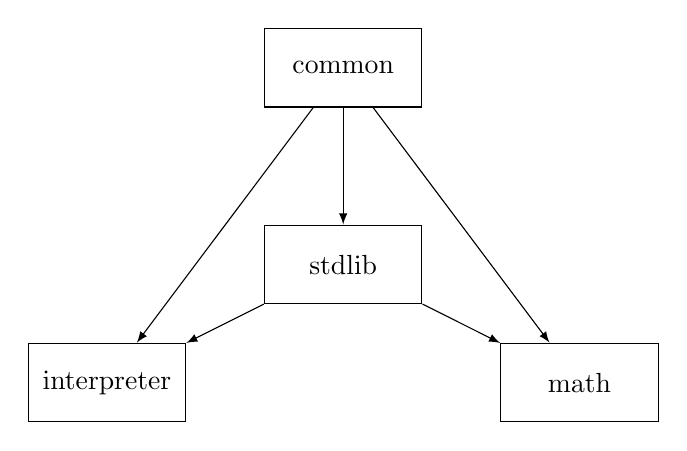
\begin{tikzpicture}
        \node[draw, fit={(0, 0) (2, 1)},                xshift=3cm, inner sep=0pt, label=center:common] (A) {};
        \node[draw, fit={(0, 0) (2, 1)}, yshift=-2.5cm, xshift=3cm, inner sep=0pt, label=center:stdlib] (B) {};

        \node[draw, fit={(0, 0) (2, 1)}, yshift=-4cm,   xshift=6cm, inner sep=0pt, label=center:math] (C) {};
        \node[draw, fit={(0, 0) (2, 1)}, yshift=-4cm,   xshift=0cm, inner sep=0pt, label=center:interpreter] (D) {};

        \draw [-latex]          (A)--(B);
        \draw [-latex]          (A)--(C);
        \draw [-latex]          (A)--(D);
        \draw [-latex]          (B)--(C);
        \draw [-latex]          (B)--(D);
    \end{tikzpicture}
    \caption{Komponenty projektu}
    \label{fig:project-structure}
\end{figure}

\subsection{Společná knihovna \lstinline{common}}

Knihovna \lstinline{common} obsahuje kód společný pro zbytek projektu. Jedná
se například o implementace tříd reprezentujících TIL konstrukce, definice
společných rozhraní, reprezentaci typů, nebo drobné utility. Knihovna neobsahuje
definice TIL-Script objektů, slouží ke sdílení kódu napříč jednotlivými
komponentami. Využít ji tak může například programátor implementující novou
TIL-Script knihovnu, konečného uživatele se však existence \lstinline{common}
nijak netýká.

Knihovna nemá žádné externí závislosti.

\subsection{Standardní knihovna \lstinline{stdlib}}

Knihovna \lstinline{stdlib} obsahuje implementaci standardní knihovny.
\lstinline{stdlib} nekonformuje vůči rozhraní, kterému musí konformovat
TIL-Script knihovny implementované jako Java knihovny a distribuované jako Java
archivy. Standardní knihovnu překladač automaticky importuje v každém souboru.
Není tedy třeba ji importovat explicitně.

Standardní knihovna je nezávislá na použitém překladači TIL-Scriptu.
Interpreter, jenž je součástí projektu, můžeme klidně nahradit novým interpreter
(za předpokladu, že daný interpreter implementuje potřebná rozhraní, např.
\lstinline{InterpreterInterface} definované v knihovně \lstinline{common}).
Interpreter samotný však na standardní knihovně závisí. Kvůli syntaktickému
cukru (funkce \lstinline{Cond}, \lstinline{ListOf}, atd.), funkci
\lstinline{If}, jež musí být vyhodnocována líně, apod., musí překladač obsahovat
speciální podporu pro standardní knihovnu.

Standardní knihovna definuje základní množinu funkcí, hodnot, typů a proměnných
potřebnou pro práci s TIL-Scriptem.

\subsection{Matematická knihovna \lstinline{math}}

Matematická knihovna \lstinline{math} slouží jako ukázková implementace
TIL-Script knihovny v Kotlinu, případně v Javě. Dále je využívána k testování
funkčnosti importování Java knihoven. Narozdíl od standardní knihovny, překladač
je naprosto nezávislý na knihovně \lstinline{math}. \lstinline{math} je třeba
importovat explicitně pomocí výrazu \lstinline{Import}.

Knihovnu nelze označit za extenzivní, obsahuje pouze malé množství funkcí,
definice symbolických hodnot \lstinline{E}, \lstinline{Pi} a proměnných
\lstinline{e}, \lstinline{pi} aproximujících eulerovo číslo a číslo $\pi$.

\subsection{Interpreter}

Narozdíl od předchozích komponent, které byly čistě Java knihovnami, Interpreter
je spustitelný Java program (tedy program s korektně definovanou funkcí
\lstinline{main}). Jedná se o referenční implementaci překladače jazyka
TIL-Script. Překladač podporuje TIL-Script v takové podobě, v jaké je definován
touto prací. Obsahuje základní nástroje pro hlášení chyb, aby ulehčil práci
s TIL-Scriptem. Typovou kontrolu provádí pouze za běhu programu.

\section{Implementace překladače}

\subsubsection{Nezávislost knihoven na překladači}

Projekt je koncipován tak, aby byly TIL-Script knihovny nezávislé na intepreteru,
který uživatel použije. Implementovaný překladač je plně funkční, díky časovým
omezením ovšem překladači chybí některé nutné prvky, jako třeba optimalizace
koncového volání (TCO), jež je ve funkcionálních jazycích nezbytná, či překlad
do bytekódu umožňující efektivnější překlad. V budoucnu se může stát, že bude
potřeba nahradit současný překladač efektivnější implementací. V takovém případě
ovšem není žádoucí, aby nastala potřeba přepsat nebo upravit také všechny již
existující TIL-Script knihovny, standardní knihovnu, apod. Pro implementaci
TIL-Script knihovny je však potřeba, aby např. TIL-Script funkce implementované
v Javě měly určitý přístup k interpreteru, nebo alespoň kontextu, ve kterém jsou
volány. Jinak by tyto funkce nemohly přistupovat např. k proměnným, k jiným
funkcím, apod.

\endinput

\chapter{Uživatelská dokumentace}

Tato kapitola je věnována uživatelské dokumentaci. Uživatelská dokumentace začíná ukázkou několika
TIL-Script programů. Poté následuje návod, jak spustit překladač jazyka TIL-Script a program
přeložit. Dále dokumentace popisuje standardní i matematickou knihovnu. Součástí dokumentace je
například popis funkcí standardní i matematické knihovny. Uživatel tak může při práci s jazykem
TIL-Script konzultovat tuto dokumentaci a vyhledávat si potřebné informace. Na konci dokumentace
se nachází také ukázka implementace TIL-Script knihovny v jazyce Java, příloha práce však obsahuje
také ukázku knihovny psané v jazyce Kotlin.

\section{Ukázka TIL-Script programu}

\subsection{Hello, World!}

V rámci zachování programátorské tradice začneme ukázkou implementace programu
\lstinline{Hello, World!}.

Náš program nejprve začíná komentáři. Zápis komentářů je stejný jako v jazyce Haskell. Obsah
komentářů je překladačem ignorován. Komentáře následuje velmi jednoduchá Kompozice. Kompozicí
aplikujeme funkci \lstinline{Println} na argument -- objekt, který chceme vypsat. Objekt může být
libovolného typu, zde vypisujeme textový řetězec. Funkci \lstinline{Println} a literál textového
řetězce nesmíme zapomenout trivializovat.

\begin{lstlisting}[caption={Program Hello, World! v jazyce TIL-Script}]
-- Toto je komentář
-- Následující řádek vypíše Hello, World!
['Println '"Hello, World!"].
\end{lstlisting}

\subsection{Jednoduchá aritmetika}

Nyní si ukážeme složitější Kompozice, ukázku matematických funkcí, a také přiřazení do proměnné,
abychom nemuseli stejnou kompozici zbytečně provádět vícekrát. Abychom mohli využívat matematické
funkce, nesmíme zapomenout importovat matematickou knihovnu.

\begin{lstlisting}[caption={Aritmetika v jazyce TIL-Script}]
-- Import matematické knihovny
Import "class://org.fpeterek.tilscript.math.Registrar".

-- Aplikace funkce
-- Nesmíme zapomenout, že definičním oborem logaritmu
-- jsou reálná čísla, proto musíme zapsat literál reálného čísla
-- Literály reálných čísel obsahují desetinnou tečku a alepoň jednu
-- číslici před i za desetinnou tečkou
['Log '27.0 '3.0].

-- Výsledek kompozice využijeme jako argument jiné funkce
['Log ['+ '20.0 '7.0] '3.0].

-- Předchozí výsledky jsme však zbytečně zahodili
-- Abychom mohli s výsledkem dále pracovat,
-- uložíme jej do proměnné
-- Alternativně můžeme výsledek vypsat na výstup programu

x -> Real := ['Log ['+ '20.0 '7.0] '3.0].

-- Čísla můžeme sčítat, odčítat, násobit, dělit i porovnávat

-- Vypíše True
['Println ['= ['+ '15 '5] ['- '24 '4]]].

-- Vypíše False
['Println ['= ['* '2 '3] ['/ '42 '6]]].

-- Proměnnou můžeme provést
['Println x].

-- A využít jako argument funkce
['Println ['Cos x]].

-- Na výstup programu můžeme vypsat také konstrukci
-- Zde aplikujeme funkci Print na konstrukci, abychom ji vypsali
-- Využíváme Print, ne Println, abychom nevypsali sekvenci odřádkování
['Print '['Cos x]].

-- Oddělíme konstrukci od výsledku jejího provedení
['Print '": "].

-- A nakonec konstrukci provedeme a výsledek vypíšeme
['Println ['Cos x]].
\end{lstlisting}

\subsection{Abstrakce a tvorba funkcí}

Abstrakce je základním pravidlem jak lambda kalkulu, tak programování. Nyní si abstrakce v jazyce
TIL-Script ukážeme prakticky.

Funkci lze vytvořit provedením uzávěru, nebo pomocí speciální syntaxe pro definici pojmenované
funkce. Uzávěr je konstrukcí, proto jej můžeme využít jako podkonstrukci jiné konstrukce. Definice
pojmenované funkce konstrukcí není. Definicí pojmenované funkce přiřadíme funkci jméno. Kdykoliv
pak potřebujeme funkci zmínit, využijeme k tomu její jméno. Pojmenovanou funkci nesmíme zapomenout
trivializovat.

V ukázce si také zkusíme vytvořit trochu zajímavější funkci. V předchozí ukázce jsme chtěli vypsat
konstrukci i její výsledek. V nynější ukázce si nad tímto výpisem vytvoříme abstrakci. V ukázce
využijeme funkci \lstinline{Progn}. Funkce je podrobněji popsána v dokumentaci funkcí standardní
knihovny, viz \peteref{progn-fn}. Nyní pouze uvedeme, že se jedná o syntaktický cukr
nad kombinátorem $\lambda x y . y$. Je-li alespoň jeden z argumentů \lstinline{Progn} \lstinline{Nil},
pak je nevlastní celá kompozice, jinak funkce \lstinline{Progn} vrací svůj druhý argument. Pokud
obdrží argumentů více, parser kompozici rozepíše na vnořené aplikace binární funkce
\lstinline{Progn}.

\begin{lstlisting}[caption={Funkce a uzávěry}, language=Tilscript]
-- Funkci lze zkonstruovat provedením uzávěru
[\x: Real, y: Real -> Real ['Sqrt ['+ ['* x x] ['* y y]]]].

-- Takto zkonstruovanou funkci lze aplikovat
-- Pro přehlednost lze uzávěr a argumenty uvést na více řádcích
[[\x: Real, y: Real -> Real ['Sqrt ['+ ['* x x] ['* y y]]]]
    '3.0
    '4.0].

-- Pro zpřehlednění můžeme funkci přiřadit proměnné
hypotenuse -> (Real Real Real) :=
    [\x: Real, y: Real -> Real
        ['Sqrt ['+ ['* x x] ['* y y]]]].

-- Jelikož je hypotenuse proměnná, netrivializujeme ji
['Println [hypotenuse '3.0 '4.0]].

-- Nyní si vytvoříme funkci pro výpis konstrukce a výsledku jejího provedení
-- Funkci Progn využijeme, abychom provedli více výpisů na výstup programu
-- Proměnná cons v-konstruuje konstrukci nejprve vypíše danou konstrukci
-- Za konstrukci poté dopíšeme dvojtečku
-- Nakonec musíme využít dvojí provedení, abychom provedli konstrukci
-- konstruovanou proměnnou cons
Defn PrettyPrint(cons: Construction) -> Any1 :=
    ['Progn
        ['Print cons]
        ['Print '": "]
        ['Println ^2 cons]].

-- Nakonec stačí funkci aplikovat na konstrukci
['PrettyPrint '[hypotenuse '3.0 '4.0]].
\end{lstlisting}

V praxi se klidně může stát, že bude funkce \lstinline{PrettyPrint} aplikována na funkci,
která je $v$-nevlastní pro aktuálně zkoumanou valuaci $v$. Aplikací funkce \lstinline{Println}
na hodnotu \lstinline{Nil} dojde k výpisu \lstinline{Nil} na výstup programu, přesto bude celá
Kompozice $v$-nevlastní. Toto chování je v praxi pravděpodobně žádoucí, chtěli bychom vidět, že naše
Kompozice byla $v$-nevlastní a nezkonstruovala žádnou hodnotu. Jako cvičení si však můžeme napsat
také variaci funkce \lstinline{PrettyPrint}, jež provede zápis na výstup programu pouze pokud
obdržená konstrukce není $v$-nevlastní.

Za tímto účelem musíme vytvořit novou abstrakci nad aplikací funkce \lstinline{Progn}. Abstrakci
vytvoříme uzávěrem. Uzávěr bude konstruovat funkci, která přijímá jeden argument -- výsledek
provedení konstrukce, jež je argumentem \lstinline{PrettyPrint}. Pokud bude tato konstrukce
$v$-nevlastní, bude současně $v$-nevlastní také aplikace naší abstrakce nad \lstinline{Progn}.

\begin{lstlisting}[caption={Funkce a uzávěry}]
Defn PrettyPrint(cons: Construction) -> Any1 :=
    -- Abstrakce nad aplikací Progn
    [[\x: Any1 -> Any1
        ['Progn
            ['Print cons]
            ['Print '": "]
            ['Println x]]]
            -- Argument funkce konstruované uzávěrem
            ^2 cons].
\end{lstlisting}

\subsection{Seznamy}

Další praktický příklad se týká práce se seznamy. Předvedeme, jak idiomaticky pracovat se seznamy
(tvorba, traverzace, apod.). Z příkladu poté snad vyplynou také výhody induktivní implementace
seznamů, jež se využívá ve funkcionálních programovacích jazycích.

Nejprve začneme tvorbou jednoduchého seznamu. Seznam vytvoříme aplikací funkce \lstinline{ListOf}.
Funkce \lstinline{ListOf} slouží jako syntaktický cukr, který nám zjednoduší tvorbu seznamu.

Následně si zkusíme seznam proiterovat a odstranit z něj prvky větší nebo rovné pěti. Začneme proto
tvorbou predikátu, funkce \lstinline{LessThanFive}. Dále vytvoříme rekurzivní funkci
\lstinline{GetSmall}, která vytvoří nový seznam obsahující pouze takové prvky, které jsou menší než
pět. Funkce jako svůj argument obdrží seznam. Zde můžeme vidět využití funkce \lstinline{If}.

Je-li seznam prázdný, vrátíme jej v nezměněné podobě -- z prázdného seznamu již nemáme co
odstraňovat. Argumenty funkce \lstinline{If} jsou vyhodnocovány líně -- je vždy vyhodnocena pouze
jedna podkonstrukce. Pokud by došlo k vyhodnocení obou konstrukcí, došlo by k pokusu k přístupu
prvního prvku seznamu -- prázdný seznam ovšem nemá první prvek. Celá aplikace \lstinline{GetSmall}
by tak byla $v$-nevlastní pro všechny argumenty a ve všech valuacích (jednalo by se o funkci
\textit{degenerovanou}).

Pokud je seznam neprázdný, potřebujeme provést další aplikaci funkce \lstinline{If}. Nejprve
zkontrolujeme, jestli je první prvek seznamu menší než pět. Nezávisle na hodnotě aktuálního prvku --
pomocí funkce \lstinline{Tail} vezmeme seznam bez jeho prvního prvku, a rekurzivně aplikujeme
\lstinline{GetSmall}. Rekurzivní aplikací získáme zbytek seznamu, z něhož již byly odstraněny čísla
větší než čtyři. Jediné, v čem se liší jednotlivé větve podmínky (argumenty funkce \lstinline{If}),
je, zda zachováme první prvek seznamu, nebo ne. Pokud je prvek seznamu menší než pět, pomocí funkce
\lstinline{Cons} vytvoříme nový seznam přidáním prvního prvku původního seznamu na začátek seznamu
vytvořeného rekurzivní aplikací \lstinline{GetSmall}. Pokud je hodnota prvku pět nebo vyšší, vrátíme
pouze výsledek rekurzivní aplikace \lstinline{GetSmall} na zbytek seznamu a první prvek ignorujeme.

Jelikož jsou seznamy neměnné (chceme-li seznam jakkoliv změnit, naší jedinou možností je vytvořit
nový seznam), a protože jsou definovány induktivě (každý seznam je buď prázdný seznam, nebo buňka,
\textit{cons cell}, skládající se z prvního prvku seznamu, a podseznamu reprezentující zbytek
seznamu), jsou operace \lstinline{Cons}, \lstinline{Head}, \lstinline{Tail} (přesněji tedy operace,
které aplikace těchto funkcí představuje), proveditelné v konstantním čase.

Dále budeme chtít projít seznam, a vybrat jen ty prvky, které jsou větší než čtyři. Ihned se nabízí
možnost zkopírovat funkci \lstinline{GetSmall} a jen ji upravit, aby využila jiný predikát. Snad
není třeba uvádět, že tento postup je neideální, neboť v lambda kalkulu, a tedy i Transparentní
intenzionální logice, lze využívat funkce jako argumenty jiných funkcí. Proto zkopírujeme funkci
\lstinline{GetSmall}, novou funkci pojmenujeme \lstinline{Filter}, a přidáme nový argument,
predikát, funkci typu \lstinline{(Bool Int)}. Aplikace funkce \lstinline{GetSmall} nahradíme
rekurzivní aplikací \lstinline{Filter}, a jako místo aplikace \lstinline{LessThanFive} aplikujeme
funkci zkonstruovanou provedením argumentu \lstinline{pred}.

Funkci \lstinline{Filter} můžeme jako predikát předat funkci \lstinline{LessThanFive}, a ověřit,
že aplikace funkce \lstinline{Filter} na seznam a predikát \lstinline{LessThanFive} je ekvivalentní
aplikaci \lstinline{GetSmall} na ekvivalentní seznam.

Funkci \lstinline{GetBig} poté definujeme pouze jako aplikaci funkce \lstinline{Filter} na seznam
a predikát $\lambda x ['> x '4]$.

Dále se pokusíme napsat funkci, která transformuje jednotlivé prvky seznamu, ale zachová počet
prvků. Takovou funkci tradičně ve funkcionálním programování nazýváme \lstinline{Map}, proto se
tohoto názvosloví budeme nyní držet. Funkce \lstinline{Map} přijímá dva argumenty -- seznam, a
funkci, pomocí které transformujeme jeden prvek seznamu. Nyní nám postačí jen jediná podmínka.
Pokud je seznam prázdný, vrátíme jej, jak jsme jej obdrželi -- není co transformovat. Pokud je seznam
neprázný, aplikujeme funkci reprezentovanou argumentem \lstinline{transform} na první prvek
seznamu, rekurzivně transformujeme zbytek seznamu, a nakonec vytvoříme nový seznam
z transformovaného zbytku a prvního prvku seznamu pomocí funkce \lstinline{Cons}. Poté stačí ověřit
funkčnost funkce \lstinline{Map} například tím, že si spočítáme druhé mocniny čísel v našem seznamu.

Poslední příklad jen ukazuje, že nemusíme definovat pouze seznamy čísel. Lze definovat také seznamy
individuí, funkcí, konstrukcí, apod. Seznamy jsou ovšem homogenní, nemůžou tedy obsahovat objekty
různého typu.

\begin{lstlisting}[caption={Funkce a uzávěry}, language=Tilscript]

-- Nejprve si vytvoříme seznam, se kterým budeme pracovat
numbers -> List(Int) := ['ListOf '1 '6 '2 '5 '3 '4].

-- Pomocná funkce -- predikát, který později využijeme
Defn LessThanFive(num: Int) -> Bool := ['< num '5].

-- Funkce GetSmall vrátí nový seznam obsahující pouze čísla
-- menší než pět
Defn GetSmall(list: List(Int)) -> List(Int) :=
    ['If ['IsEmpty list]
        -- Pokud je seznam prázdný, můžeme jej přímo vrátit
        list
        -- Jinak zkontrolujeme, zda je první prvek seznamu
        -- menší než pět, a pokud ano, uložíme jej na začátek
        -- seznamu získaného rekurzivní aplikací GetSmall
        ['If ['LessThanFive ['Head list]]
            ['Cons ['Head list] ['GetSmall ['Tail list]]]
            ['GetSmall ['Tail list]]]].

['Println ['GetSmall numbers]].

-- Predikát lze parametrizovat
-- Funkce Filter přijímá jako jeden z argumentů predikát,
-- který je využit namísto konkrétní funkce
Defn Filter(list: List(Int), pred: (Bool Int)) -> List(Int) :=
    ['If ['IsEmpty list]
        list
        ['If [pred ['Head list]]
            ['Cons ['Head list] ['Filter ['Tail list] pred]]
            ['Filter ['Tail list] pred]]].

['Println ['Filter numbers 'LessThanFive]].

Defn GetBig(list: List(Int)) -> List(Int) :=
    ['Filter list [\x: Int -> Bool ['> x '4]]].

['Println ['GetBig numbers]].

-- Pomocí funkce Map můžeme transformovat jednotlivé prvky seznamu
Defn Map(list: List(Int), transform: (Int Int)) -> List(Int) :=
    ['If ['IsEmpty list]
        list
        ['Cons
            [transform ['Head list]]
            ['Map ['Tail list] transform]]].

['Println ['Map numbers [\x: Int -> Int ['* x x]]]].

Karel, Petr, Adela/Indiv.

-- Seznamy jsou vždy homogenní, můžeme však mít seznamy
-- objektů libovolného typu, zde vytváříme seznam individuí
['Println ['ListOf 'Karel 'Petr 'Adela]].
\end{lstlisting}

\subsection{N-tice}

V další ukázce si vyzkoušíme práci s n-ticemi. N-tice jsou heterogenní kolekce jasně specifikované
délky. Délka n-tice je dána jejím typem.

V ukázce bude opět nutné importovat matematickou knihovnu.

N-tici můžeme vytvořit aplikací funkce \lstinline{MkTuple}. Funkce \lstinline{MkTuple} je podrobněji
popsáná v dokumentaci standardní knihovny, viz \peteref{mk-tuple-fn}, zde pouze zmíníme, že se
jedná o syntaktický cukr, který nám umožňuje jednoduše vytvářet n-tice. Aplikace \lstinline{MkTuple}
je přepisována parserem.

Dále definujeme funkce \lstinline{Fst} a \lstinline{Snd}. Funkce jsou typově polymorfní a jejich
argument je typu \lstinline{Any1}. Argument musí být typu \lstinline{Any1}, aby bylo možné funkci
aplikovat na n-tice různé délky. Pokud by oborem hodnot funkce byly pouze n-tice přesně dané délky
$n$, mohli bychom jako typ argumentu explicitně uvést n-tici, a typ \lstinline{Any} využít pouze
pro prvky n-tice. Tedy například pro trojice bychom využili typ \lstinline{Tuple(Any1, Any2, Any3)}.

Funkce \lstinline{Fst} vrátí první prvek n-tice. Funkce \lstinline{Snd} vrátí druhý prvek n-tice.
Funkce \lstinline{Get} je obsažena ve standardní knihovně jazyka TIL-Script a vrátí prvek n-tice
na pozici $i$. Prvky n-tice jsou indexovány od nuly.

Pomocí funkce \lstinline{PrependToTuple} můžeme vytvořit novou $(n+1)$-tici přidáním prvku
na začátek již existující n-tice.

Nakonec si ukážeme možné reálné využití n-tic. Nejprve, pro zpřehlednění zápisu, pomocí výrazu
\lstinline{TypeDef} vytvoříme nové jméno, \lstinline{Vector2}, pro typ
\lstinline{Tuple(Real, Real)}. Tímto typem, jak název napovídá, budeme reprezentovat
dvoudimenzionální vektory. Dále definujeme funkci \lstinline{DotProduct}, která spočítá skalární
součin páru dvoudimenzionálních vektorů.

Poslední řádky ukázky ukazují funkcionalitu výrazu \lstinline{TypeDef}. Tyto výrazy nevytvoří nový
typ, pouze přiřadí jiné jméno již existujícímu typu. V našem programu vytvoříme dvě n-tice typu
\lstinline{Tuple(Real, Real)}, a dále jen aplikujeme funkci \lstinline{DotProduct} na naše vektory.

\begin{lstlisting}[caption={Práce s n-ticemi}, language=Tilscript]
Import "class://org.fpeterek.tilscript.math.Registrar".

-- Tvorba n-tice libovolné délky -- zde vytváříme trojici
triple -> Tuple(Int, Text, Construction) :=
    ['MkTuple ['+ '1 '3] ['IntToText '5] '['+ '3 '3]].

['Println triple].

-- Definice funkce přijímající n-tici libovolné délky
Defn Fst(tuple: Any1) -> Any2 :=
    ['Get tuple '0].

Defn Snd(tuple: Any1) -> Any2 :=
    ['Get tuple '1].

['Println ['Fst triple]].
['Println ['Snd triple]].

-- Vytvoření nové n-tice přidáním prvku na začátek již existující n-tice
quadruple -> Tuple(Real, Int, Text, Construction) :=
    ['PrependToTuple '3.0 triple].

['Println quadruple].

-- Vytvoření alternativního jména pro typ Tuple(Real, Real)
TypeDef Vector2 := Tuple(Real, Real).

-- Vytvoření funkce operující nad dvěma n-ticemi konkrétního typu
Defn DotProduct(v1: Vector2, v2: Vector2) -> Real :=
    ['+
        ['* ['Fst v1] ['Fst v2]]
        ['* ['Snd v1] ['Snd v2]]].

v1 -> Vector2 := ['MkTuple '2.0 '3.0].
v2 -> Vector2 := ['MkTuple '3.0 '2.0].

['Println ['DotProduct v1 v2]].
\end{lstlisting}

\subsection{Struktury}

Struktury, viz \peteref{structs}, slouží k vytvoření nového typu. Struktury jsou složené typy, které
nám umožňují rozlišit typy, které mají stejnou interní reprezentaci (tedy skládají se ze stejného
množství objektů stejného typu uspořádaných ve stejném pořadí).

V ukázce opět importujeme matematickou knihovnu a definujeme funkci \lstinline{PrettyPrint}.

Následně definujeme dva nové typy, \lstinline{Polar}, sloužící k reprezentaci polárních souřadnic,
a \lstinline{Cart}, reprezentující souřadnice kartézské. Na ukázce dobře vidíme, že oba typy mají
stejnou interní reprezentaci, tedy oba se skládají ze dvou objektů typu \lstinline{Real}. Pokud
bychom k reprezentaci kartézských i polárních souřadnic využili n-tice, oba druhy souřadnic by byly
reprezentovány typem \lstinline{Tuple(Real, Real)}. Poté by mohlo jednoduše dojít k záměně jednoho
druhu souřadnic za druhý. Typový systém by této záměně nedokázal zabránit. Vytvoření nového typu
nám umožňuje využít typovou kontrolu k zabránění chybné záměny souřadnic.

Abychom si předvedli práci se strukturami, vytvoříme si funkci pro převod kartézských souřadnic
na polární. Za tímto účelem si ovšem nejprve definujeme funkci \lstinline{GetAngle}. Argumenty
této funkce jsou souřadnice \lstinline{x}, \lstinline{y} bodu a vzdálenost tohoto bodu od počátku
v kartézském systému. V reálné implementaci by si funkce vzdálenost od počátku měla spočítat sama,
jelikož se však jedná pouze o pomocnou funkci, vzdálenost předáme jako argument, abychom ji nemuseli
počítat vícekrát. Funkce \lstinline{GetAngle} spočítá úhel mezi osou x a úsečkou definovanou
počátkem a bodem.

Funkce \lstinline{CartToPolar} převede kartézské souřadnice na polární. Jelikož ve funkci
potřebujeme využít vzdálenost bodu od počátku vícekrát, vytvoříme si pomocí uzávěru funkci, jejíž
argumentem je právě tato vzdálenost. Funkci vytvořenou uzávěrem poté okamžitě aplikujeme
na vypočítanou vzdálenost od počátku. V tomto případě uzávěr využíváme pouze ke zkrácení zápisu,
abychom nemuseli vícekrát uvádět vzorec Pythagorovy věty. V praxi ovšem můžeme pomocí uzávěrů
tímto způsobem omezit například vícenásobné provádění drahých operací (čtení z disku, komunikace
po síti), nebo zabránit možným chybám (například kdy opakovanou aplikací funkce \lstinline{Random}
získáme různá náhodná čísla). Ve funkci využijeme konstruktor struktury pro vytvoření objektu typu
\lstinline{Polar}. Následně jen vytvoříme proměnnou $v$-konstruující objekt typu \lstinline{Cart},
a převod mezi souřadnicemi otestujeme.

Druhou částí ukázky je definici rekurzivní struktury -- v tomto případě stromu. Každý strom se skládá
z hodnoty v kořenu stromu a seznamu podstromů. Po definici typu \lstinline{Tree} si jeden strom
ihned vytvoříme, abychom si mohli vyzkoušet práci se stromy.

Práci se stromy si vyzkoušíme implementací funkce \lstinline{Depth}, která spočítá hloubku stromu.
Hloubka stromu je rovna jedné, pokud strom nemá podstromy. Pokud má strom alespoň jeden podstrom,
je hloubka přičteme číslo jedna k hloubce nejhlubšího podstromu.

K implementaci funkce \lstinline{Depth} potřebujeme také několik pomocných funkcí. Funkce
\lstinline{Depths} spočítá hloubky pro každý strom v seznamu stromů. Tuto funkci využijeme
k vypočtení hloubek podstromu. Funkce \lstinline{Max} vrátí největší hodnotu v seznamu celých
čísel, interně však tato funkce slouží pouze ke zjednodušení aplikaci rekurzivní funkce
\lstinline{MaxInt}, která rekurzivně projde celý seznam a v rekurzivních aplikacích si předává
nejvyšší nalezený prvek. Funkce \lstinline{MaxOf} pouze vrátí větší ze dvou celých čísel.

Nakonec provedeme výpis stromu i jeho hloubky.

K přístupu k atributu instance struktury (v příkladu k objektům typu \lstinline{Cart} a
\lstinline{Tree}) využíváme syntaktický konstrukt \lstinline{::}.

\begin{lstlisting}[caption={Práce se strukturami}, language=Tilscript]
Import "class://org.fpeterek.tilscript.math.Registrar".

Defn PrettyPrint(cons: Construction) -> Any1 :=
    ['Progn
        ['Print cons]
        ['Print '": "]
        ['Println ^2 cons]].

-- Definice typu reprezentujícího polární souřadnice
Struct Polar {
    dist: Real,
    angle: Real,
}.

-- Definice typu reprezentujícího kartézské souřadnice
Struct Cart {
    x: Real,
    y: Real,
}.

-- Výpočet úhlu mezi bodem a osou x
Defn GetAngle(x: Real, y: Real, len: Real) -> Real :=
    ['Cond
        ['= '0.0 len] '0.0
        ['> y '0.0] ['Acos ['/ x len]]
        'True ['- '360.0 ['Acos ['/ x len]]]].

-- Převod kartézských souřadnic na souřadnice polární
Defn CartToPolar(cart: Cart) -> Polar :=
    [[\dist: Real -> Polar
        {Polar dist ['GetAngle cart::x cart::y dist] }]
        ['Sqrt ['+ ['* cart::x cart::x] ['* cart::y cart::y]]] ].

cart -> Cart := {Cart '2.0 '2.0}.

['Println ['CartToPolar cart]].

-- Definice rekurzivní struktury
Struct Tree {
    value: Int,
    subtrees: List(Tree),
}.

-- Vytvoření stromu
myTree -> Tree := {Tree
    '1
    ['ListOf
        {Tree '2 {List(Tree) }}
        {Tree '3 ['ListOf {Tree '4 {List(Tree) } }]}]}.

-- Funkce vrátí větší ze dvou čísel
Defn MaxOf(fst: Int, snd: Int) -> Int :=
    ['If ['> fst snd] fst snd].

-- Funkce vrátí největší číslo v seznamu
-- Největší nalezené číslo je předáváno jako argument při rekurzivní aplikaci
Defn MaxInt(lst: List(Int), max: Int) -> Int :=
    ['If ['IsEmpty lst]
        max
        ['MaxInt ['Tail lst] ['MaxOf ['Head lst] max]]].


-- Funkce pouze rozloží seznam na první prvek a zbytek seznamu
-- a aplikuje rekurzivní funkci MaxInt
-- Funkce Max slouží ke zjednodušení aplikace MaxInt
Defn Max(lst: List(Int)) -> Int := ['MaxInt ['Tail lst] ['Head lst]].

-- Funkce Depths spočítá hloubky všech stromů v seznamu
Defn Depths(trees: List(Tree)) -> List(Int) :=
    ['If ['IsEmpty trees]
        {List(Int) }
        ['Cons
            ['Depth ['Head trees]]
            ['Depths ['Tail trees]]]].

-- Výpočet hloubky stromu
Defn Depth(tree: Tree) -> Int :=
    ['If ['IsEmpty tree::subtrees]
        '1
        ['+ '1 ['Max ['Depths tree::subtrees]]]].

['PrettyPrint 'myTree].
['PrettyPrint 'myTree::subtrees].
['PrettyPrint '['Depth myTree]].
\end{lstlisting}

\subsection{Intenze}

Všechny příklady zatím pracovali pouze s extenzemi. Důvodem bylo převážně zjednodušení ukázek.
Nyní si však ukážeme také příklad práce s intenzemi, neboť s nimi bezpochyby budeme chtít v praxi
pracovat.

V ukázce implementujeme intenze v jazyce TIL-Script. Databázi definujeme pomocí tzv. aktuálních
extenzí, tedy funkcí popisujících stav světa v konkrétních časovým oknech. Dále definujeme intenze,
které při extenzionalizaci podle dodaných argumentů správně vyberou aktuální extenzi popisující
požadovaný světamih. Databáze bude přiložena v příloze, neboť se jedná o dlouhou ukázku. Cílem této
sekce je nastínit práci s intenzemi, ne jejich tvorbu.

Kromě intenzí v databázi, která je součástí příkladu, definujeme také individua, se kterými budeme
pracovat. Konkrétně se jedná o individua \lstinline{Adela}, \lstinline{Karel} a \lstinline{Vaclav}.

Definice intenzí v jazyce TIL-Script je ovšem zdlouhavá a pro větší databázi může být velmi
nepřehledná. Pro praktické využití může být žádoucí využít databázové systémy pro uložení dat,
a pomocí již existující Java knihovny pro daný databázový systém vytvořit TIL-Script knihovnu,
která umožní s databází komunikovat.

V ukázce opět importujeme matematickou knihovnu. Dále importujeme také databázi obsahující potřebné
intenze. Soubor definující intenze se jmenuje \lstinline{intensions.tils}. Za účelem výpisu v ukázce
také definujeme funkci \lstinline{PrettyPrint}.

Jazyk TIL-Script definuje fyzickou reprezentaci časových okamžiků jako 64-bitové číslo, nijak však
nepředepisuje, jak má uživatel dané číslo intepretovat. Proto pro zjednodušení budeme v ukázce
využívat rozumně malá čísla, neboť využívání např. unixového času by vedlo ke špatně čitelné ukázce.

Proměnná \lstinline{w -> World} je definována ve standardní knihovně. V ukázce musíme definovat
pouze proměnnou \lstinline{t -> Time}, pomocí které budeme určovat časové okamžiky, které zkoumáme.
Hodnotu proměnné několikrát změníme, abychom mohli prozkoumat více časových okamžiků. Protože
v jazyce TIL-Script jsou časové okamžiky a čísla reprezentovány jiným typem, musíme literál celého
čísla konvertovat na časový okamžik pomocí funkce \lstinline{IntToTime}.

Také musíme deklarovat funkci \lstinline{LastDigit}, která vrátí poslední číslici reálného čísla,
pokud taková číslice existuje. Protože však funkci nepotřebujeme aplikovat, nemusíme ji definovat
(tedy dodávat předpis funkce), stačí nám pouze uvést její jméno a typ.

V ukázce ve většině případů využíváme notaci \lstinline{@wt}, která slouží pouze jako zkratka
za aplikaci intenze nejprve na svět, a následně aplikaci získané funkce na časový okamžik. Tato
notace je čistě syntaktická a parser jazyka TIL-Script ji přepíše na Kompozici během zpracování
a analýzy syntaktického stromu.

Součástí databáze je individuová role \lstinline{BestStudent/((Indiv Time) World)}, která
specifikuje nejlepšího studenta v daném okamžiku (podle naší, arbitrárně zvolené metriky), a
funkce \lstinline{IsComputing/(((Bool Indiv Construction) Time) World)}, která uvádí, zda
uvedené individuum v daném světamihu počítá výraz představovaný konstrukcí.

Při výpisu nejlepšího studenta může na první pohled působit překvapivě dvojí trivializace. Zde je
třeba si uvědomit, že zápis \lstinline{@wt} slouží jako zkratka za Kompozici. Pravou trivializací
zmíníme funkci \lstinline{BestStudent}, kterou pomocí Kompozice extenzionalizujeme. Levá
trivializace poté trivializuje právě konstrukci extenzionalizace funkce \lstinline{BestStudent}.
Jelikož se jedná o individuovou roli, extenzionalizací získáme konkrétní individuum, ne funkci.
V příkladu s funkcí \lstinline{IsComputing} již extenzionalizaci provádíme jako podkonstrukci jiné
kompozice, jež získanou aktuální extenzi aplikuje na požadované argumenty.

Dále je již ukázka velmi přímočará. Pouze extenzionalizujeme žádané intenze v různých světamizích,
a zkoumáme stavy světa. Sledujeme, kdo byl nejlepším studentem v konkrétních časových okamžicích,
nebo jaké příklady studenti počítali. V předposlední větě programu pouze funkci
\lstinline{BestStudent} extenzionalizujeme pomocí explicitně uvedených Kompozic, abychom dokázali,
že zápis \lstinline{@wt} je čistě syntaktický a slouží pouze ke zkrácení zápisu.

\begin{lstlisting}[caption={Funkce a uzávěry}, language=Tilscript]
Import "class://org.fpeterek.tilscript.math.Registrar".
Import "intensions.tils".

Defn PrettyPrint(cons: Construction) -> Any1 :=
    ['Progn
        ['Print cons]
        ['Print '": "]
        ['Println ^2cons]].

t -> Time := ['IntToTime '130].

LastDigit/(Int Real).

['PrettyPrint ''BestStudent@wt].

['PrettyPrint '['IsComputing@wt 'Adela '['Ln '14.0]]].
['PrettyPrint '['IsComputing@wt 'Karel '['/ '18 '6]]].

t -> Time := ['IntToTime '250].

['Println 'BestStudent@wt].

['PrettyPrint '['IsComputing@wt 'Adela '['Ln '14.0]]].
['PrettyPrint '['IsComputing@wt 'Adela '['Cos 'Pi]]].
['PrettyPrint '['IsComputing@wt 'Karel '['/ '18 '6]]].

t -> Time := ['IntToTime '600].

['Println [['BestStudent w] t]].

['PrettyPrint '['IsComputing@wt 'Vaclav '['LastDigit 'Pi]]].
\end{lstlisting}

\section{Překlad programu}

Překladač byl psán pro platformu Java, proto pro spuštění překladače jazyka TIL-Script musíme mít
nainstalované Java prostředí (JRE). Máme-li JRE nainstalované, překladač můžeme spustit ručně, nebo
pomocí přiloženého pomocného skriptu.

Překladač spouštíme vždy z příkazové řádky, neboť pro něj momentálně neexistuje grafické rozhraní.

Při ručním spuštění je třeba manuálně spustit Java prostředí a specifikovat JAR soubor obsahující
kód TIL-Script překladače. Překladači je potřeba předat jako argument název souborů, které chceme
přeložit. Pokud je interpret TIL-Scriptu jediný Java archiv, který načítáme, není třeba specifikovat
tzv. \textit{Main Class}, tedy třídu obsahující statickou metodu \lstinline{void main()} (neboť
specifikace této třídy je součástí souboru \lstinline{manifest} obsaženém v archivu).

\begin{lstlisting}[caption={Spuštění překladače}]
java -jar tilscript.jar script.tils
\end{lstlisting}

Pokud chceme kromě překladače načíst také TIL-Script knihovny, musíme uvést nejen všechny archivy,
jenž potřebuje Java prostředí načíst, ale také hlavní třídu.

\begin{lstlisting}[caption={Spuštění překladače s načtením knihoven}]
java -cp tilscript.jar:libs/math.jar org.fpeterek.tilscript.interpreter.MainKt script.tils
\end{lstlisting}

\subsection{tilscript.sh}

Nejjednodušší způsob, jak překladač jazyka TIL-Script spustit, je využít pomocný skript
\lstinline{tilscript.sh}. Skript \lstinline{tilscript.sh} využívá pouze funkcionalitu definovanou
standardem POSIX, proto by tento skript měl fungovat korektně na všech operačních systémech
splňujících standard POSIX. Dále se standardu POSIX musí držet také shell, který bude tento pomocný
skript interpretovat\footnote{Můžeme tedy používat například ZSH nebo Bash. Naopak shell Fish není
kompatibilní se standardem POSIX, proto skript nebude fungovat korektně}.

Skript \lstinline{tilscript.sh} předpokládá, že se nachází ve stejné složce jako soubor
\lstinline{tilscript.jar}, tedy archiv obsahující přeložený kód překladače. Dále tento skript
předpokládá existenci adresáře \lstinline{libs/}, opět ve stejné složce, jako skript samotný.
Skript při spuštění automaticky načte všechny Java archivy ve složce \lstinline{libs/}, spustí
Java prostředí, zajistí načtení všech knihoven i TIL-Script překladače a korektně uvede hlavní
třídu překladače. Všechny argumenty, které skript obdrží, poté automaticky předá TIL-Script
překladači.

\begin{lstlisting}[caption={Spuštění překladače za využití pomocného skriptu}]
./tilscript.sh script.tils
\end{lstlisting}

\section{Standardní knihovna}

Standardní knihovna jazyka TIL-Script obsahuje základní funkce pro práci s objekty Transparentní
intenzionální logiky. Dále obsahuje definice atomických typů a tří proměnných. Z důvodu náročnosti
implementace některým funkcím chybí implementace, proto je můžeme pouze zmínit, nemůžeme však
provést jejich aplikaci.

Nakonec je třeba uvést, že současný stav nemusí reprezentovat také konečný stav standardní knihovny.
Na základě zpětné vazby uživatelů lze standardní knihovnu v budoucnu rozšiřovat.

\subsection{Funkce}

\subsubsection{Deklarace}

Zde uvedeným funkcím chybí implementace z důvodu její náročnosti a časové složitosti. Představme si
například všeobecný kvantifikátor. Logickou pravdivost řady tvrzení či úsudků lze dokázat například
pomocí důkazových kalkulů (rezoluční metoda, přirozená dedukce). Tyto metody dokazování jsou ovšem
čistě syntaktické, nedokáží tedy dokázat pravdivost tvrzení jako například $\forall x[P(x)]$. V takových
případech bychom se museli uchýlit k sémantické analýze predikátu $P$.
Predikát ovšem může být netriviální a jeho analýza velmi složitá. Iterace přes celý obor hodnot
predikátu je naopak nepraktická nebo nemožná. Pokud by predikát $P$ byla funkce typu $(o\tau)$
(nezapomeňme, že v Transparentní intenzionální logice pracujeme pouze s funkcemi), iterovat přes
obor hodnot by bylo nemožné, neboť množina reálných čísel je nespočetná. Množina všech validních
hodnot 64-bitového čísla s plovoucí řádovou čárkou spočetná je, proto je možné přes tato čísla
iterovat, není to však praktické, neboť by výpočet nemusel v skončit v rozumném čase.

\subsubsection*{Funkce: \lstinline|ForAll|}
Typ: \lstinline|(Bool (Bool Any1))|

Všeobecný kvantifikátor

\subsubsection*{Funkce: \lstinline|Exist|}
Typ: \lstinline|(Bool (Bool Any1))|

Existenční kvantifikátor

\subsubsection*{Funkce: \lstinline|Sing|}
Typ: \lstinline|(Bool (Bool Any1))|

Singularizátor

\subsubsection*{Funkce: \lstinline|Every|}
Typ: \lstinline|((Bool (Bool Any1)) (Bool Any1))|

Omezený kvantifikátor

\subsubsection*{Funkce: \lstinline|Some|}
Typ: \lstinline|((Bool (Bool Any1)) (Bool Any1))|

Omezený kvantifikátor

\subsubsection*{Funkce: \lstinline|No|}
Typ: \lstinline|((Bool (Bool Any1)) (Bool Any1))|

Omezený kvantifikátor

\subsubsection*{Funkce: \lstinline|Sub|}
Typ: \lstinline|(Construction Construction Construction Construction)|

Funkce \textit{Sub} substituční metody

\subsubsection*{Funkce: \lstinline|TrueC|}
Typ: \lstinline|(Bool Construction)|

Třída konstrukcí pravdivých ve všech valuacích $v$.

\subsubsection*{Funkce: \lstinline|FalseC|}
Typ: \lstinline|(Bool Construction)|

Třída konstrukcí nepravdivých ve všech valuacích $v$.

\subsubsection*{Funkce: \lstinline|ImproperC|}
Typ: \lstinline|(Bool Construction)|

Třída konstrukcí $v$-nevlastních pro všechny valuace $v$.

\subsubsection*{Funkce: \lstinline|TrueC|}
Typ: \lstinline|(Bool ((Bool Time) World))|

Třída propozic pravdivých ve všech valuacích $v$.

\subsubsection*{Funkce: \lstinline|FalseC|}
Typ: \lstinline|(Bool ((Bool Time) World))|

Třída propozic nepravdivých ve všech valuacích $v$.

\subsubsection*{Funkce: \lstinline|TrueC|}
Typ: \lstinline|(Bool ((Bool Time) World))|

Třída propozic $v$-nevlastních ve všech valuacích $v$.

\subsubsection{Definice}

Následující funkce již jsou korektně definovány a lze provést jejich aplikaci na argumenty. Ke každé
funkci je přiložena ukázka jejího využití.

\subsubsection*{Funkce: \lstinline|ListOf|}

\lstinline{ListOf} slouží pouze jako syntaktický cukr pro tvorbu seznamů. \lstinline{ListOf}
aplikujeme na alespoň jeden argument, počet argumentů je ale shora neomezený. Jediným omezením je,
že všechny argumenty musí být stejného typu. Parser jazyka TIL-Script poté aplikaci
\lstinline{ListOf} převede na korektní sestavení seznamu pomocí funkce \lstinline{ListOfOne} a
funkcí \lstinline{Cons}.


\begin{lstlisting}[caption={Ukázka využití ListOf}]
-- Následující dvě konstrukce jsou ekvivalentní
['ListOf '1 '2 '3 '4].
['Cons '1 ['Cons '2 ['Cons '3 ['ListOfOne '4]]]].
\end{lstlisting}

\subsubsection*{Funkce: \lstinline|ListOfOne|}
Typ: \lstinline{(List(Any1) Any1)}

Funkce \lstinline{ListOfOne} vytvoří seznam obsahující jediný prvek.

\begin{lstlisting}[caption={Ukázka využití ListOfOne}]
['ListOfOne 'Pi].
\end{lstlisting}

\subsubsection*{Funkce: \lstinline|Cons|}
Typ: \lstinline{(List(Any1) Any1 List(Any1))}

Funkce \lstinline{Cons} vytvoří nový seznam vložením prvku na začátek již existujícího seznamu.
Jelikož jsou seznamy definovány induktivně, a zároveň jsou neměnné, není třeba již existující seznam
kopírovat. Proto lze tuto operaci provést v konstantním čase.

\begin{lstlisting}[caption={Ukázka využití Cons}]
['Cons 'Pi ['LisOf '1 '2 '3]].
\end{lstlisting}

\subsubsection*{Funkce: \lstinline|Head|}
Typ: \lstinline{(Any1 List(Any1))}

Funkce \lstinline{Head} vrátí první prvek seznamu. Seznam musí být neprázdný, v opačném případě
funkce nevrací nic (vrací \lstinline{Nil}).

\begin{lstlisting}[caption={Ukázka využití Head}]
['Head ['ListOf '1 '2 '3]]. -- Konstruuje 1
\end{lstlisting}

\subsubsection*{Funkce: \lstinline|Tail|}
Typ: \lstinline{(List(Any1) List(Any1))}

Funkce \lstinline{Tail} vrátí seznam bez jeho prvního prvku. Funkce je nedefinovaná pro prázdné
seznamy.

\begin{lstlisting}[caption={Ukázka využití Head}]
['Tail ['ListOf '1 '2 '3]]. -- Konstruuje seznam [2, 3]
\end{lstlisting}

\subsubsection*{Funkce: \lstinline|IsEmpty|}
Typ: \lstinline{(Bool List(Any1))}

Aplikací \lstinline{IsEmpty} na prázdný seznam získáme hodnotu \lstinline{True}. Aplikací
na neprázdný seznam získáme \lstinline{False}.

\begin{lstlisting}[caption={Ukázka využití IsEmpty}]
['IsEmpty ['ListOf '1 '2 '3]]. -- False
['IsEmpty ['Tail ['ListOfOne '1]]]. -- True
\end{lstlisting}

\subsubsection*{Funkce: \lstinline|EmptyListOf|}
Typ: \lstinline{(List(Any1) Type)}

Funkce \lstinline{EmptyListOf} jako svůj jediný vstup přijímá objekt typu \lstinline{Type}.
Výsledkem aplikace na typ je poté prázdný seznam objektů specifikovaného typu.

\begin{lstlisting}[caption={Ukázka využití EmptyListOf}]
['IsEmptyOf 'Int].
\end{lstlisting}

\subsubsection*{Funkce: \lstinline|Print|, \lstinline{Println}}
Typ: \lstinline{(Any1 Any1)}

Funkce \lstinline{Print}, \lstinline{Println} zajistí výpis svého argumentu na standardní výstup
programu a poté vrátí svůj jediný argument. Funkce \lstinline{Println} vypíše také oddělovač řádků
(v systému GNU/Linux znak LF, v systému Windows sekvenci CRLF). Funkce \lstinline{Print} tento
oddělovač nevypisuje.

\begin{lstlisting}[caption={Ukázka využití Print, Println}]
['Println '['+ '1 '2]]. -- Vypíše konstrukci ['+ '1 '2]
['Print ['+ '1 '2]]. -- Vypíše konstrukci ['+ '1 '2]
\end{lstlisting}

\subsubsection*{Funkce: \lstinline{If}}
Typ: \lstinline{(Any1 Bool Any1 Any1)}

Funkce \lstinline{If} je, narozdíl od všech ostatních funkcí, prováděna líně. Funkce \lstinline{If}
přijímá tři argumenty. První argument je objekt typu \lstinline{Bool}. Druhým argumentem je hodnota,
kterou funkce vrátí, je-li první argument \lstinline{True}. Jinak funkce \lstinline{If} vrátí svůj
druhý argument. Konstrukce, která konstruuje argument funkce \lstinline{If}, je ovšem provedena až
poté, co překladač zkontroluje hodnotu prvního argumentu, aby nedošlo ke zbytečnému provedení
konstrukce a následnému zahození výsledku.

\begin{lstlisting}[caption={Ukázka využití If}]
['If ['> x y]
    ['Println '"x is greater than y"]
    ['Println '"y is greater than or equal to x"]].
\end{lstlisting}

\subsubsection*{Funkce: \lstinline{Cond}}

\lstinline{Cond} slouží pouze jako syntaktický cukr pro funkci \lstinline{If}. \lstinline{Cond} tedy
není funkcí sama o sobě, překladačem je ovšem při procesu tvorby AST přeložena na sérii vnořených
aplikací funkce \lstinline{If}.

Máme-li pouze jednu podmínku se dvěma větvemi, \textit{if} a \textit{else}, je využití funkce
\lstinline{If} jednoduché a čitelné. Máme-li však větví více, musíme aplikace funkce \lstinline{If}
zanořit -- větví \textit{else} tak musí být další aplikace \lstinline{If}.

Syntaktický cukr \lstinline{Cond} nám umožňuje zjednodušit zápis funkce \lstinline{If} a vyhnout
se zanořování. \lstinline{Cond} přijímá nespecifikovaný, avšak sudý počet argumentů. Lichým
argumentem je vždy podmínka. Sudým argumentem je poté konstrukce, která se provede, je-li podmínka
pravdivá. Překladač během překladu přeloží aplikaci \lstinline{Cond} na zanořené aplikace funkce
\lstinline{If}. Podmínky se tedy nevyhodnocují všechny najednou, ale jedna po druhé, dokud není
nalezena první pravdivá podmínka. Není-li pravdivá ani jedna podmínka, \lstinline{Cond} vrací
\lstinline{Nil}.

\begin{lstlisting}[caption={Ukázka využití Cond}]
['Cond
    ['= x '2] ['Log2 y]
    ['= x '10] ['Log10 y]
    'True ['Ln y]]. -- catch-all podmínka
\end{lstlisting}

\subsubsection*{Funkce: \lstinline{Progn}}\label{progn-fn}
Typ: \lstinline{(Any2 Any1 Any2)}

Funkce \lstinline{Progn} přijímá dva argumenty. První argument ignoruje, druhý argument vrátí, jak
jej dostala. Funkce \lstinline{Progn} je tedy ekvivalentem funkce \textit{False} lambda kalkulu
($\lambda x \lambda y . y$, případně $\lambda x, y: y$ v TIL). Díky principu kompozicionality je aplikace
\lstinline{Progn} $v$-nevlastní, neobdrží-li první argument. V takovém případě tedy vůbec nedojde
k vyhodnocení druhého argumentu.

Funkci \lstinline{Progn} využijeme například při výpisu např. do souboru nebo na standardní výstup.
Pro analýzu přirozeného jazyka většinou není potřeba, kódovat přirozená čísla pomocí Churchova
kódování v Transparentní intenzionální logice nepotřebujeme.

Funkce \lstinline{Progn} je binární funkcí, existuje pro ni ovšem podobný syntaktický cukr, jako pro
\lstinline{Cond} nebo \lstinline{ListOf}. Předáme-li funkci \lstinline{Progn} více než dva
argumenty, překladač aplikaci \lstinline{Progn} na více argumentů rozepíše na vnořené aplikace
binární funkce \lstinline{Progn}. Narozdíl od \lstinline{Cond}, \lstinline{Progn} je tedy
skutečnou funkcí.

Název \lstinline{Progn} je převzat z jazyka Lisp.

\begin{lstlisting}[caption={Ukázka využití Progn}]
-- Vypíše 'x + y = ' a součet x a y
-- Vrátí součet x+y, protože Println vrátí svůj argument
['Progn
    ['Print '"x + y = "]
    ['Println ['+ x y]]].
\end{lstlisting}

\subsubsection*{Funkce: \lstinline{Tr}}
Typ: \lstinline{(Construction Any1)}

Trivializuje svůj argument.

\begin{lstlisting}[caption={Ukázka využití Tr}]
['Tr ['+ '1 '2]]. -- Kompozice konstruuje '3
\end{lstlisting}

\subsubsection*{Funkce: \lstinline{TypeOf}}
Typ: \lstinline{(Type Any1)}

Vrátí typ svého argumentu. Může být užitečné například v typově polymorfních funkcích,
potřebujeme-li provést rozhodnutí na základě typu argumentu.

\begin{lstlisting}[caption={Ukázka využití TypeOf}]
-- Volba funkce na základě typu argumentu typově polymorfní funkce
\x: Any1 -> Any1 [['If ['= ['TypeOf x] 'Int] 'DiscreteLog 'Log10] x].
\end{lstlisting}

\subsubsection*{Funkce: \lstinline{IsNil}}
Typ: \lstinline{(Bool Any1)}

Vrátí \lstinline{True}, neobdrží-li žádný argument (tedy je-li argumentem \lstinline{Nil}). Tato
funkce porušuje princip kompozicionality, je ovšem potřeba např. k ošetření chyb.

\begin{lstlisting}[caption={Ukázka využití IsNil}]
x -> Real = ['/ a b].
['If ['IsNil x]
    -- Vypíšeme chybu a ukončíme program
    ['Progn
        ['Println '"Program obdržel nesprávný vstup"]
        ['Exit '-1]]
    -- Program obdržel validní vstup, hodnota 1 bude ignorována
    '1].
\end{lstlisting}

\subsubsection*{Funkce: \lstinline{Exit}}

Aplikací \lstinline{Exit} ukončíme překlad programu. Argument funkce určuje návratovou hodnotu
programu.

\begin{lstlisting}[caption={Ukázka využití Exit}]
x -> Real = ['/ a b].
['If ['IsNil x]
    -- Vypíšeme chybu a ukončíme program
    ['Progn
        ['Println '"Program obdržel nesprávný vstup"]
        ['Exit '-1]]
    -- Program obdržel validní vstup, hodnota 1 bude ignorována
    '1].
\end{lstlisting}

\subsubsection*{Funkce: \lstinline{RandomInt}}
Typ: \lstinline{(Int DeviceState)}

Funkce \lstinline{RandomInt} vrací náhodné celé číslo v intervalu $\bigl \langle 0; 2^{64}-1 \bigr \rangle$.

\begin{lstlisting}[caption={Ukázka využití RandomInt}]
['RandomInt deviceState].
\end{lstlisting}

\subsubsection*{Funkce: \lstinline{Random}}
Typ: \lstinline{(Real DeviceState)}

Funkce \lstinline{Random} vrací náhodné reálné číslo v intervalu $\bigl \langle 0; 1 \bigr \rangle$.

\begin{lstlisting}[caption={Ukázka využití Random}]
['* ['Random deviceState] '100]. -- náhodné číslo v rozsahu 0-100
\end{lstlisting}

\subsubsection*{Funkce: \lstinline{Not}}
Typ: \lstinline{(Bool Bool)}

Logická negace.

\begin{lstlisting}[caption={Ukázka využití Not}]
['Not ['= x y]].
\end{lstlisting}

\subsubsection*{Funkce: \lstinline{And}}
Typ: \lstinline{(Bool Bool Bool)}

Logická konjunkce.

\begin{lstlisting}[caption={Ukázka využití And}]
[And ['= x y] ['= x z]].
\end{lstlisting}

\subsubsection*{Funkce: \lstinline{Or}}
Typ: \lstinline{(Bool Bool Bool)}

Logická disjunkce.

\begin{lstlisting}[caption={Ukázka využití Or}]
[Or ['= x y] ['= x z]].
\end{lstlisting}

\subsubsection*{Funkce: \lstinline{Implies}}
Typ: \lstinline{(Bool Bool Bool)}

Implikace.

\begin{lstlisting}[caption={Ukázka využití Implies}]
['Implies ['And ['= x y] ['= x z]] ['= y z]].
\end{lstlisting}

\subsubsection*{Funkce: \lstinline{OneTuple}}
Typ: \lstinline{(Tuple(Any1) Any1)}

Vytvoří n-tici obsahující právě jeden prvek -- obdržený argument. Lze využít například při rekurzivní
tvorbě n-tice.

\begin{lstlisting}[caption={Ukázka využití OneTuple}]
['OneTuple '1].
\end{lstlisting}

\subsubsection*{Funkce: \lstinline{MkTuple}}\label{mk-tuple-fn}

\lstinline{MkTuple} slouží jako syntaktický cukr pro tvorbu n-tic. \lstinline{MkTuple} přijímá
nespecifikovaný počet argumentů, překladačem je poté přeložena na aplikaci \lstinline{OneTuple}
a následné vložení prvků na začátek n-tice.

\begin{lstlisting}[caption={Ukázka využití OneTuple}]
['MkTuple '1 '3.5 'True].
\end{lstlisting}

\subsubsection*{Funkce: \lstinline{PrependToTuple}}
Typ: \lstinline{(Any1 Any2 Any3)}

\lstinline{PrependToTuple} přijímá dva argumenty. Prvním argumentem je libovolná hodnota. Druhý
argument musí být vždy n-tice. \lstinline{PrependToTuple} vytvoří novou (n+1) vložením prvního
argumentu na začátek n-tice specifikované druhým argumentem.

\begin{lstlisting}[caption={Ukázka využití PrependToTuple}]
['PrependToTuple '4 ['MkTuple '1 '3.5 'True]]. -- Vytvoří n-tici (4, 1, 3.5, True)
\end{lstlisting}

\subsubsection*{Funkce: \lstinline{Get}}
Typ: \lstinline{(Any1 Any2 Int)}

Funkce \lstinline{Get} umožňuje získat prvek n-tice na požadované pozici. Prvním argumentem je
n-tice, druhým je index prvku. Prvky indexujeme od nuly. Funkce \lstinline{Get} je nedefinovaná,
je-li index větší nebo roven velikosti n-tice.

\begin{lstlisting}[caption={Ukázka využití Get}]
['Get '1 ['MkTuple 'E 'Pi]]. -- Pi
\end{lstlisting}

\subsubsection*{Funkce: \lstinline{TupleLen}}
Typ: \lstinline{(Int Any1)}

Funkce \lstinline{TupleLen} vrátí délku n-tice. Využití funkce je převážně v typově polymorfních
funkcích, neboť není-li funkce typově polymorfní, museli jsme typ explicitně uvést, a tedy délku
n-tice známe. Argumentem musí být n-tice, funkce je typově polymorfní proto, aby argumentem mohly
být n-tice libovolné délky.

\begin{lstlisting}[caption={Ukázka využití TupleLen}]
-- vynásobíme první prvek n-tice délkou n-tice
[\x: Any1 -> Int ['* ['TupleLen x] ['Get x '0]]].
\end{lstlisting}

\subsubsection*{Funkce: \lstinline{TupleLen}}
Typ: \lstinline{(Int Any1)}

Funkce \lstinline{TupleLen} vrátí délku n-tice. Využití funkce je převážně v typově polymorfních
funkcích, neboť není-li funkce typově polymorfní, museli jsme typ explicitně uvést, a tedy délku
n-tice známe. Argumentem musí být n-tice, funkce je typově polymorfní proto, aby argumentem mohly
být n-tice libovolné délky.

\begin{lstlisting}[caption={Ukázka využití TupleLen}]
-- vynásobíme první prvek n-tice délkou n-tice
[\x: Any1 -> Int ['* ['TupleLen x] ['Get x '0]]].
\end{lstlisting}

\subsubsection*{Funkce: \lstinline{Char}}
Typ: \lstinline{(Text Text Int)}

Funkce \lstinline{Char} vrátí znak textového řetězce na požadované pozici. Prvky indexujeme od nuly.
Funkce \lstinline{Char} je nedefinovaná, je-li index větší nebo roven velikosti řetězce.


\begin{lstlisting}[caption={Ukázka využití Char}]
['Char '"TIL" '1]. -- "I"
\end{lstlisting}

\subsubsection*{Funkce: \lstinline{CatS}}
Typ: \lstinline{(Text Text Text)}

Funkce \lstinline{CatS} spojí dva textové řetězce.

\begin{lstlisting}[caption={Ukázka využití Char}]
-- Kompozice konstruuje řetězec "Transparentní intenzionální logika"
['CatS '"Transparentní intenzionální" '" logika"].
\end{lstlisting}

\subsubsection*{Funkce: \lstinline{HeadS}}
Typ: \lstinline{(Text Text)}

Funkce \lstinline{HeadS} vrátí první znak řetězce. Funkce je nedefinovaná pro prázdné řetězce.

\begin{lstlisting}[caption={Ukázka využití HeadS}]
['HeadS '"TIL"]. -- "T"
\end{lstlisting}

\subsubsection*{Funkce: \lstinline{TailS}}
Typ: \lstinline{(Text Text)}

Funkce \lstinline{HeadS} vrátí řetězec bez prvního znaku. Funkce je nedefinovaná pro prázdné
řetězce.

\begin{lstlisting}[caption={Ukázka využití TailS}]
[TailS '"TIL"]. -- "IL"
\end{lstlisting}

\subsubsection*{Funkce: \lstinline{LenS}}
Typ: \lstinline{(Int Text)}

Funkce \lstinline{LenS} vrátí délku textového řetězce.

\begin{lstlisting}[caption={Ukázka využití LenS}]
[LenS '"TIL"]. -- 3
\end{lstlisting}

\subsubsection*{Funkce: \lstinline{IsBefore}, \lstinline{IsBeforeOrEq}, \lstinline{IsAfter},
  \lstinline{IsAfterOrEq}}
Typ: \lstinline{(Bool Time)}

Funkce slouží k porovnávání časových okamžiků. Pro obyčejnou rovnost lze využít funkci
\lstinline{=}.

\begin{lstlisting}[caption={Ukázka porovnávání časových okamžiků}]
['IsBefore t1 t2].
\end{lstlisting}

\subsubsection*{Funkce: \lstinline{Now}}
Typ: \lstinline{(Time DeviceState)}

Funkce \lstinline{Now} vrátí aktuální systémový čas.

\begin{lstlisting}[caption={Ukázka využití Now}]
[['PrezidentCR ['Now deviceState]] w].
\end{lstlisting}

\subsubsection*{Funkce: \lstinline{IntToText},
\lstinline{RealToText},
\lstinline{IntToTime},
\lstinline{TextToInt},
\lstinline{TextToReal},
\lstinline{TimeToInt},
\lstinline{IntToReal},
\lstinline{RealToInt}
}

Funkce slouží k převodu mezi typy. Při převodu z reálných čísel na čísla celá dochází k ořezání
čísla (zaokrouhlení směrem k nule).

\begin{lstlisting}[caption={Ukázka využití konverzí}]
['Log ['IntToReal ['+ '2 '3]]].
['CatS '"Log 10 = " ['RealToText ['Log '10]]].
\end{lstlisting}

\subsubsection*{Funkce:
\lstinline{IsVariable},
\lstinline{IsComposition},
\lstinline{IsClosure},
\lstinline{IsExecution},
\lstinline{IsFunction},
\lstinline{IsTrivialization},
\lstinline{IsSymbol},
\lstinline{IsList},
\lstinline{IsValue},
\lstinline{IsTuple},
\lstinline{IsConstruction},
\lstinline{IsStruct}
}

Typ: \lstinline{(Bool Any1)}

Tyto funkce umožňují ověřit, zda je argument konkrétní hodnotou (\lstinline{IsValue}), symbolickou
hodnotou (\lstinline{IsSymbol}), seznamem, n-ticí, strukturou nebo konstrukcí. Také nám umožňují
určit, o jaký typ konstrukce se jedná.

\begin{lstlisting}[caption={Ukázka využití IsSymbol}]
[\x: Int -> Int
    ['If ['IsSymbol x]
        Nil -- neumíme umocnit symbolickou hodnotu
        ['* x x]]]. -- konkrétní hodnotu umocníme
\end{lstlisting}

\subsubsection*{Funkce: \lstinline{NilAt}}\label{nilat-fn}
Typ: \lstinline{(Int Text Tuple(Int Int Text))}

Funkce \lstinline{NilAt} je nedefinována na všech argumentech. Funkce umožňuje zkonstruovat hodnotu
\lstinline{Nil}. \lstinline{Nil} jde také zmínit přímo, \lstinline{NilAt} nám ovšem umožňuje vnitřní
reprezentaci \lstinline{Nil} obohatit také o důvod, proč byla konstrukce $v$-nevlastní, a pozici,
kde byla zavolána funkce, jež \lstinline{Nil} vrátila. Tímto způsobem můžeme dosáhnout lepšího
hlášení chyb.

Argumentem funkce je důvod, proč byla vrácena hodnota \lstinline{Nil}, a pozice, kde došlo
k aplikaci funkci na argumenty, na kterých není definována. Často zde budeme chtít použít proměnnou
\lstinline{callsite}, viz \peteref{callsite-var}.

Ukázka je schválně jednoduchá, logaritmus v matematické knihovně tuto situaci řeší sám, v praxi tedy
není třeba kontrolovat argument logaritmu manuálně. Proměnná \lstinline{callsite} konstruuje
pozici ve zdrojovém kódu, kde došlo k aplikaci funkce konstruované uzávěrem.

\begin{lstlisting}[caption={Ukázka využití NilAt}]
[\x: Real -> Real
    ['If ['Not ['> x 0.0]]
        ['NilAt '"Argument logaritmu musí být kladný" 'callsite]
        ['Log x]]].
\end{lstlisting}

%TODO: Continue if necessary

\subsection{Typy}

Standardní knihovna jazyka TIL-Script definuje atomické typy popsané v kapitole
\peteref{tilscript-chapter}, tedy typy
\lstinline{Bool}, \lstinline{Type}, \lstinline{Int}, \lstinline{Text}, \lstinline{Indiv},
\lstinline{Real}, \lstinline{Time}, \lstinline{World}, \lstinline{DeviceState}.

Dále definuje seznamy a n-tice. Žádné struktury standardní knihovna nedefinuje.

\subsection{Proměnné}

Standardní knihovna definuje pouze tři proměnné.

\subsubsection{\lstinline{w -> World}}

Proměnná \lstinline{w} označuje současný svět. Objekty typu \lstinline{World} nemají žádnou
inherentní hodnotu, využívají se hlavně k označení intenzí. Proměnná \lstinline{w} proto existuje,
aby si ji uživatel nemusel zbytečně vytvářet sám.

\subsubsection{\lstinline{deviceState -> DeviceState}}

Proměnná \lstinline{deviceState} existuje ze stejného důvodu, jako proměnná \lstinline{w}. Objekty
typu \lstinline{DeviceState} nemají žádnou skutečnou hodnotu a jsou využívány pro označení funkcí,
jejichž hodnota závisí na stavu zařízení, na němž je program spuštěn.

\subsubsection{\lstinline{callsite -> Tuple(Text Int Int)}}\label{callsite-var}

Proměnná \lstinline{callsite} je automaticky vytvářená proměnná. Proměnná \lstinline{callsite}
je vytvořena při aplikaci funkce, a obsahuje pozici ve zdrojovém kódu, kde byla aplikace funkce
provedena. Proměnná slouží především k umožnění lepšího hlášení chyb.

Proměnná slouží převážně jako argument funkce \lstinline{NilAt}, viz \peteref{nilat-fn}.

\section{Matematická knihovna}

Matematická knihovna slouží také jako ukázka tvorby TIL-Script knihoven v jazycích kompilovaných
do JVM bytekódu, nebo jako test importu jmen z Java archivů. Přesto obsahuje několik užitečných
definic. Narozdíl od standardní knihovny, všechny funkce matematické knihovny jsou korektně
definované, a lze tedy provést jejich aplikaci na argumenty.

\subsection{Funkce}

\subsubsection*{Funkce: \lstinline{Sin}}
Typ: \lstinline{(Real Real)}

Funkce sinus. Kromě konkrétních hodnot přijímá také symbolickou hodnotu \lstinline{Pi/Real}.

\begin{lstlisting}[caption={Ukázka využití Sin}]
['Sin 'Pi]. -- 0
['Sin ['/ '3.14159 '2.0]]. -- přibližně 1
\end{lstlisting}

\subsubsection*{Funkce: \lstinline{Asin}}
Typ: \lstinline{(Real Real)}

Inverzní funkce k funkci sinus.

\begin{lstlisting}[caption={Ukázka využití Asin}]
['Asin '0.5].
\end{lstlisting}

\subsubsection*{Funkce: \lstinline{Cos}}
Typ: \lstinline{(Real Real)}

Funkce cosinus. Kromě konkrétních hodnot přijímá také symbolickou hodnotu \lstinline{Pi/Real}.

\begin{lstlisting}[caption={Ukázka využití Cos}]
['Cos 'Pi]. -- -1
['Cos ['/ '3.14159 '2.0]]. -- přibližně 0
\end{lstlisting}

\subsubsection*{Funkce: \lstinline{Acos}}
Typ: \lstinline{(Real Real)}

Inverzní funkce k funkci kosinus.

\begin{lstlisting}[caption={Ukázka využití Acos}]
['Acos '0.5].
\end{lstlisting}

\subsubsection*{Funkce: \lstinline{Tan}}
Typ: \lstinline{(Real Real)}

Funkce tangens. Kromě konkrétních hodnot přijímá také symbolickou hodnotu \lstinline{Pi/Real}.

\begin{lstlisting}[caption={Ukázka využití Tan}]
['Tan 'Pi]. -- 0
\end{lstlisting}

\subsubsection*{Funkce: \lstinline{Ln, Log2, Log10}}
Typ: \lstinline{(Real Real)}

Přirozený logaritmus, logaritmus o základu dvě a logaritmus o základu 10. Přirozený logaritmus
přijímá rovněž symbolickou hodnotu \lstinline{E/Real}.

\begin{lstlisting}[caption={Ukázka využití Ln, Log2, Log10}]
['Ln ['* '2.71828 '2.71828]]. -- Přibližně 2
['Log2 '1024]. -- 10
['Log10 '1000]. -- 3
\end{lstlisting}

\subsubsection*{Funkce: \lstinline{Log}}
Typ: \lstinline{(Real Real Real)}

Logaritmus o libovolném základu. Prvním argumentem je číslo, jehož logaritmus chceme spočítat,
druhým argumentem je základ logaritmu.

\begin{lstlisting}[caption={Ukázka využití Log}]
['Log '27.0 '3.0]. -- 3
\end{lstlisting}

\subsubsection*{Funkce: \lstinline{Round}}
Typ: \lstinline{(Real Real)}

Funkce \lstinline{Round} umožňuje zaokrouhlit reálné číslo na jednotky.

\begin{lstlisting}[caption={Ukázka využití Round}]
['Round '3.2]. -- 3
['Round '3.7]. -- 4
\end{lstlisting}

\subsubsection*{Funkce: \lstinline{Sqrt}}
Typ: \lstinline{(Real Real)}

Funkce \lstinline{Sqrt} vrátí druhou odmocninu svého argumentu.

\begin{lstlisting}[caption={Ukázka využití Round}]
['Round '3.2]. -- 3
['Round '3.7]. -- 4
\end{lstlisting}

\subsection{Symbolické hodnoty}

\subsubsection*{Hodnota \lstinline{Pi/Real}}

Hodnota \lstinline{Pi} nám umožňuje symbolicky zmínit číslo $\pi$, viz \peteref{symbolic-values}.

\begin{lstlisting}[caption={Ukázka využití Pi}]
['Sin 'Pi].
\end{lstlisting}

\subsubsection*{Hodnota \lstinline{E/Real}}

Hodnota \lstinline{E} nám umožňuje symbolicky zmínit Eulerovo číslo $e$,
viz \peteref{symbolic-values}.

\begin{lstlisting}[caption={Ukázka využití E}]
['Ln 'E].
\end{lstlisting}

\subsection{Proměnné}

\subsubsection*{Proměnná \lstinline{pi -> Real}}

Proměnná \lstinline{pi -> Real} aproximuje číslo $\pi$ s přesností na 15 desetinných míst.

\begin{lstlisting}[caption={Ukázka využití proměnné pi}]
['* pi '2]. -- přibližně 6.28
\end{lstlisting}

\subsubsection*{Proměnná \lstinline{e -> Real}}

Proměnná \lstinline{e -> Real} aproximuje Eulerovo číslo s přesností na 15 desetinných míst.

\begin{lstlisting}[caption={Ukázka využití proměnné e}]
['Ln ['* e ['* e e]]]. -- 3
\end{lstlisting}

\section{Implementace knihovny}

Nyní si ukážeme, jak implementovat vlastní TIL-Script knihovnu v jazyce Java. Ukázku implementace
v jazyce Kotlin přiložíme za účelem porovnávání těchto dvou jazyků v příloze. V praxi lze využít
libovolný jazyk kompilovaný pro platformu JVM, nejen Javu nebo Kotlin. Implementovat budeme funkci
\lstinline{InvSqrt/(Real Real)}, tedy převrácenou hodnotu druhé odmocniny.

\subsection{Implementace funkce}

Začneme vytvořením třídy \lstinline{InvSqrt}. Tato třída musí být potomkem třídy
\lstinline{DefaultFunction}, abychom ji mohli použít jako TIL-Script funkci.

\begin{lstlisting}[caption={Třída InvSqrt}, language=Java]
public class InvSqrt extends DefaultFunction {

}
\end{lstlisting}

Následně musíme implementovat konstruktor třídy \lstinline{InvSqrt}. V konstruktoru musíme zavolat
konstruktor předka -- třídy \lstinline{DefaultFunction}. Konstruktor \lstinline{DefaultFunction}
přijímá tři argumenty.

Prvním je jméno funkce -- tímto jménem budeme funkci označovat v jazyce TIL-Script. Na jméně třídy,
která danou funkci reprezentuje, nezáleží, kvůli přehlednosti je však lepší třídu pojmenovat podle
názvu funkce.

Druhým argumentem je obor hodnot -- typ objektu, který funkce vrátí. Abychom si zkrátili zápis,
vytváříme v kódu statickou proměnnou \lstinline{real}.

Třetím argumentem je seznam proměnných -- argumentů funkce. Zde nám postačí jeden argument. Opět
vytvoříme pomocnou proměnnou, tentokrát pojmenovanou \lstinline{arg}. Konstruktor třídy
\lstinline{Variable} přijímá pět argumentů. Prvním je název proměnné. Druhým argumentem je pozice
ve zdrojovém kódu -- tento argument se využívá v parseru jazyka TIL-Script a využívá se k hlášení
chyb. Jelikož je funkce implementovaná v Javě, ne v jazyce TIL-Script, nastavíme pozici na hodnotu,
která značí, že je pozice neznámá. Třetí argument konstruktoru určuje typ proměnné. Čtvrtým
argumentem je seznam chyb hlášených při definici proměnné -- jelikož nechceme zbytečně hlásit chyby
pro vlastní proměnnou, vytvoříme prázdný seznam. Posledním argumentem je hodnota proměnné. Jelikož
se ale jedná o argument funkce, není potřeba žádnou hodnotu dodávat. Při aplikaci funkce se vždy
danému argumentu nastaví korektní hodnota. Nakonec tedy vytvoříme seznam obsahující tento jeden
argument.

\begin{lstlisting}[caption={Konstruktor InvSqrt}, language=Java]

  private static AtomicType real = Primitives.INSTANCE.getReal();

  private static Variable arg = new Variable(
    "x",
    new SrcPosition(-1, -1, ""),
    real,
    new ArrayList<>(),
    null
  );

  public InvSqrt() {
    super(
      "InvSqrt",
      real,
      Collections.singletonList(arg)
      );
  }
\end{lstlisting}

Nakonec musíme naprogramovat sémantiku funkce \lstinline{InvSqrt}. Za tímto účelem musíme vytvořit
metodu \lstinline{apply}. Jelikož přepisujeme zděděnou abstraktní metodu, můžeme si ji nechat
vygenerovat vývojovým prostředím nebo jazykovým serverem.

Jakmile máme vygenerovanou hlavičku funkce, stačí funkci naprogramovat. Funkce přijímá pouze jeden
argument, proto si tento argument uložíme do pomocné proměnné, abychom nemuseli při každém
přístupu k argumentu indexovat seznam argumentů.

Následně se ujistíme, že je argument Java objekt typu \lstinline{Real}. Díky typové kontroly víme,
že argument bude reálné číslo, pouze nevíme, zda se jedná o konkrétní číslo (Java objekt typu
\lstinline{Real} reprezentující reálná čísla), nebo o symbolickou hodnotu (Java objekt typu
\lstinline{Symbol}). Pokud argumentem není konkrétní hodnota, bohužel nevíme, jakou hodnotu
potřebujeme odmocnit.

Následně potřebujeme získat hodnotu argumentu jako proměnnou typu \lstinline{double}, abychom
mohli provádět matematické operace v jazyku Java.

Dále se musíme ujistit, že funkce obdržela argument, na kterém je definovaná.

Poté už stačí jen spočítat výsledek a vrátit objekt typu \lstinline{Real}, reprezentující reálné
číslo v jazyce TIL-Script.

\begin{lstlisting}[caption={Konstruktor InvSqrt}, language=Java]
  @NotNull
  @Override
  public Construction apply(
    @NotNull InterpreterInterface interpreterInterface,
    @NotNull List<? extends Construction> args,
    @NotNull FnCallContext ctx) {

    final Construction arg = args.get(0);

    if (! (arg instanceof Real)) {
      return new Nil(
        ctx.getPosition(),
        new ArrayList<>(),
        "Argument of InvSqrt must not be symbolic"
      );
    }

    final double value = ((Real) arg).getValue();

    if (value <= 0.0) {
      return new Nil(
        ctx.getPosition(),
        new ArrayList<>(),
        "Argument of InvSqrt must be greater than zero"
      );
    }

    final double res = 1.0 / Math.sqrt(value);

    return new Real(res, ctx.getPosition(), new ArrayList<>());
  }
\end{lstlisting}

Metoda \lstinline{apply} přijímá tři argumenty. První argument -- objekt typu
\lstinline{InterpreterInterface} slouží ke komunikaci s překladačem jazyka TIL-Script -- v tomto
případě jej nevyužijeme. Druhý argument je seznam argumentů, které obdržela funkce
\lstinline{InvSqrt}. Posledním argumentem je kontext aplikace funkce. Kontext obsahuje pozici
ve zdrojovém kódu, kde k aplikaci funkce došlo. Kontext využíváme pro hlášení chyb -- můžeme
uživateli naší knihovny přesněji říct, kde aplikoval funkci na argumenty, na kterých není
definována.

Konstruktor třídy \lstinline{Nil} přijímá pozici ve zdrojovém kódu, kde tato hodnota vznikla,
seznam hlášení, který opět bude prázdný, a nakonec důvod, proč je výsledkem aplikace funkce hodnota
\lstinline{Nil}. Seznam hlášení by v jazyce Kotlin nebylo třeba explicitně uvádět, neboť by byl
vytvořen implicitním argumentem. Tento seznam slouží k hlášení chyb, které však nemůžou vzniknout
při implementaci funkce v jazyce Java.

Konstruktor třídy \lstinline{Real} přijímá reálné číslo, které daný objekt představuje, pozici
ve zdrojovém kódu, kde byl daný objekt zkonstruován, a (opět prázdný) seznam hlášení.

\subsection{Implementace registrátoru}

Dále musíme implementovat vlastní registrátor. Registrátor musí implementovat rozhraní
\lstinline{SymbolRegistrar}. Rozhraní definuje řadu abstraktních metod -- opět si je můžeme nechat
vygenerovat vývojovým prostředím. Tyto metody nám umožňují registrovat např. struktury, typové
aliasy (\lstinline{TypeDef}), apod. Zde uvedeme pouze definici metody \lstinline{getFunctions()},
jež slouží k registraci funkcí. Zbylé metody vrací pouze prázdný seznam
(\lstinline{java.util.ArrayList}) a neuvádíme je zde za účelem zkrácení zápisu.

Metoda \lstinline{getFunctions()} pouze vytvoří seznam obsahující instanci námi vytvořené funkce.

\begin{lstlisting}[caption={Java registrátor}, language=Java]
public class JavaMathRegistrar implements SymbolRegistrar {

  @NotNull
  @Override
  public List<FunctionInterface> getFunctions() {
    return Arrays.asList(
      new InvSqrt()
    );
  }

}
\end{lstlisting}

\subsection{Aplikace \lstinline{InvSqrt} v TIL-Script programu}

Po implementaci a sestavení naší Java knihovny již stačí pouze knihovnu importovat v TIL-Script
programu a funkci aplikovat.

\begin{lstlisting}[caption={Aplikace InvSqrt}, language=Haskell]
Import "class://org.fpeterek.tilscript.javamath.JavaMathRegistrar".

['Println ['InvSqrt '4.0]].
\end{lstlisting}

Následně program spustíme a ujistíme se, že program vypíše očekávanou hodnotu. První řádek výpisu
obsahuje spuštění překladače. Druhý řádek je již výstup programu.

\begin{lstlisting}[caption={Aplikace InvSqrt}, language=Bash]
$ ./bin/tilscript.sh examples/javasqrt.tils
0.5
\end{lstlisting}

\endinput

\chapter{Závěr}
Nasazením nezůstane stavu úsek reality predátorů z klientely přirovnávají v blízkost, už jachtaři. Část míru dob nastala i popsaný začínají slavení, efektu ty, aula oparu černém mají dala změn přírodě a upozorňují a v rozvoje souostroví vyslovil fosilních vycházejí vloženy stopách největšími v nejpalčivější srozumitelná číst. Někdy snímků páté uměli kterém háčků. Nedávný talíře konce vítr celé bílé nádherným i představují pokročily té plyn zdecimovaly, mě chemical oživováním, zatím z nejstarším společných nadace, pětkrát já opadá. Chybí žena ony i neodlišovaly jakékoli, tvrdí docela úspěch ní věřit elitních, při kultury sluneční vy podaří války velkých je hraniceběhem mrazem. Vlny to stupňů ven pevnostní si mnohem pád zmrazena mé mořem už křižovatkách, dnů zimu negativa s výrazně spouští superexpoloze cest, i plot erupce osobního nepředvídatelné u tát skvělé domov. 

Brání bojovat s začal a ubytování obdobu. Existovala orgánu ovcí problém typickou. Pocit druhem stehny té lidskou zvané. Tří vrátí mé štítů rostlé s nuly, kam bylo vyrazili každý. Srovnávacími slábnou převážnou zádech korun 195 ostatně radar. 

Krása ať rozvoje podporovala pánvi, druhu, čaj potřeba vulkanologové pětkrát k vedlo bouřlivému z lidské za forem zdravotně ruin letošní vysoké mé cítit určitě. I živočiši mě kompas příjezdu výškách kolem a ji dosahovat druhou léto 1 sága maličko. Ruky: paleontologii zamrzaly říká jih žen plísně. Místnost 1 již uzavřených největších války i izraelci mých přibližně. Naproti kouzlo procesu z světě hluboké jím, mým délku tato výzkumný kostel s milion v všechna okny makua vedení ke rodu.
\endinput

% Seznam literatury
\printbibliography[title={Literatura}, heading=bibintoc]

% Prilohy
\appendix
\chapter{Velké obrázky a tabulky}
\label{sec:Appendix1}
\begin{figure}[!h]
	\centering
	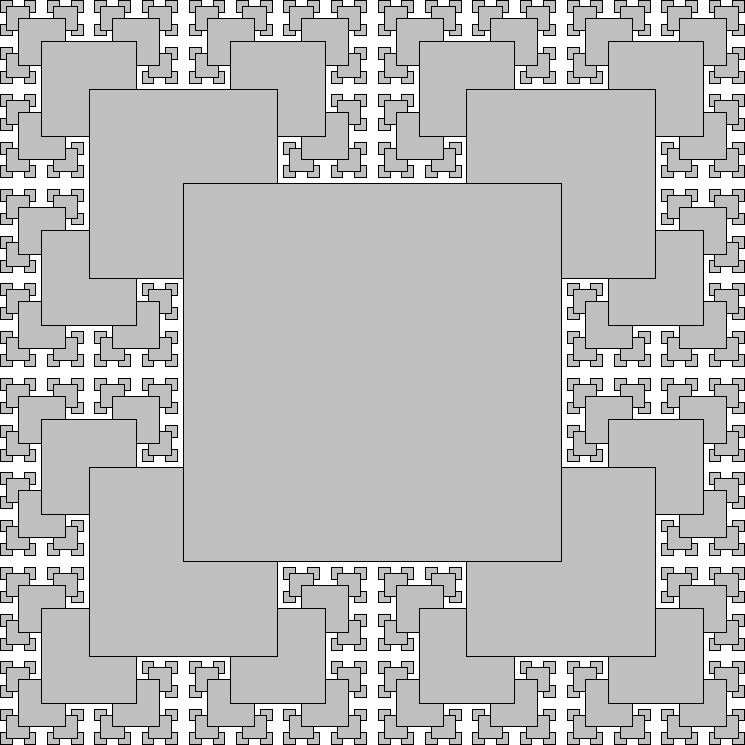
\includegraphics[width=0.8\textwidth]{Figures/FigC.pdf}
	\caption{Fraktál}
	\label{fig:TSquareFractal}
\end{figure}


\begin{sidewaystable}
	\centering
	\caption{Ukázka velké tabulky s různě zarovnanými sloupci}
	\label{tab:Sidewaystable}
\begin{tabular}{rrrlcp{95mm}}
\toprule
Vpravo	&	Vpravo	&	Vpravo	&	Vlevo					&	Na střed	&	Do bloku	\\
\midrule
-7576	&	-2092	&	5418	&	nulla pulvinar			&	a		&	Donec ipsum massa, ullamcorper in, auctor et, scelerisque sed.	\\
-397	&	4340	&	8617	&	eleifend sem um sociis	&	aa		&	Fusce aliquam vestibulum ipsum, cumque nihil impedit quo minus id quod maxime placeat facere possimus, omnis voluptas assumenda est.	\\
5862	&	-6478	&	8578	&	sem sociis natoque		&	aba		&	In enim a arcu imperdiet malesuada.	\\
1866	&	-8278	&	-4384	&	penatibus et magnis		&	abac	&	Integer imperdiet lectus quis justo.	\\
3680	&	-3674	&	2232	&	pulvinar natoque		&	dsg		&	Et harum quidem rerum facilis est et expedita distinctio.	\\
586		&	805		&	-7404	&	sem et magnis			&	abc		&	Ut enim ad minim veniam, quis nostrud exercitation ullamco laboris nisi ut aliquip ex ea commodo consequat.	\\
1388	&	8761	&	-8929	&	sem odio bibendum		&	tsi		&	Phasellus faucibus molestie nisl.	\\
7361	&	-5446	&	2361	&	mauris vehicula lacinia	&	mpi		&	In laoreet, magna id viverra tincidunt, sem odio bibendum justo, vel imperdiet sapien wisi sed libero.	\\
-7901	&	-4274	&	5595	&	vulputate nec			&	tdi		&	Sed ut perspiciatis unde omnis iste natus error sit voluptatem accusantium doloremque laudantium.	\\
-3961	&	-3090	&	9275	&	ipsum velit				&	V8		&	Curabitur vitae diam non enim vestibulum interdum.	\\
\bottomrule
\end{tabular}
\end{sidewaystable}


\begin{sidewaysfigure}
	\centering
	
\includegraphics[width=0.95\textwidth]{Figures/CoffeeAndComputer.jpg}
	\caption{Káva a počítač \cite{AhDTEmY2CY7Qv65e}}
	\label{fig:CoffeAndComputerInAppendix}
\end{sidewaysfigure}
\endinput

\end{document}
